\documentclass[manuscript,review,anonymous,nonacm,screen]{acmart}
\usepackage{graphicx}\graphicspath{{../figures/}}
\usepackage{array}\usepackage{colortbl}\usepackage{longtable}\usepackage{subcaption}\usepackage{enumitem}
\definecolor{g}{RGB}{26,152,80}\definecolor{a}{RGB}{254,224,139}\definecolor{r}{RGB}{215,48,39}
\newcommand{\PROVIDER}{an institutional vLLM API}
\newcommand{\REPO}{a public repository (URL omitted for anonymous review)}
\newcommand{\corpustabref}{Table~\ref{tab:full}}
\newcommand{\sttwotabref}{the companion review}
% auto-generated - do not edit by hand (see analysis/make_figures.py)
\newcommand{\Nstudies}{217}
\newcommand{\Ndomains}{29}
\newcommand{\Nvalidated}{8}
\newcommand{\Npromising}{60}
\newcommand{\Nmixed}{108}
\newcommand{\Ncaution}{39}
\newcommand{\Nunreliable}{2}
\newcommand{\Pctreliable}{31}
\newcommand{\Pctproblematic}{19}
\newcommand{\Nnumeric}{29}
\newcommand{\Nprimary}{206}
\newcommand{\Nsecondary}{11}
\newcommand{\Ngreen}{8}
\newcommand{\Namber}{19}
\newcommand{\Nred}{2}
\newcommand{\OAretrieved}{1500}
\newcommand{\OAunique}{957}
\newcommand{\OAtopical}{165}
\newcommand{\Webhits}{472}
\newcommand{\Webunique}{304}
\newcommand{\Nassessed}{263}
\newcommand{\Nexclscreen}{967}
\newcommand{\Crossdup}{31}
\newcommand{\Meanrel}{3.15}
\newcommand{\Nparity}{15}
% auto-generated
\newcommand{\STN}{55}
\newcommand{\STaugment}{36}
\newcommand{\STreplace}{14}
\newcommand{\STsimulate}{5}
\newcommand{\STtension}{38}
\newcommand{\STcritical}{8}
\newcommand{\STenabling}{9}
\newcommand{\SThci}{22}
\newcommand{\STmethods}{15}
\newcommand{\STrelaugment}{3.17}
\newcommand{\STrelreplace}{3.07}
\newcommand{\STrelsim}{2.8}
\newcommand{\STincluded}{55}
\newcommand{\SToa}{857}
% auto-generated
\newcommand{\STHRn}{15000}
\newcommand{\STHRdatasets}{5}
\newcommand{\STHRmodels}{6}
\newcommand{\STHRpass}{6}

% auto-generated by results_table1b.py
\newcommand{\ONEmodels}{4}
\newcommand{\ONEpanel}{\texttt{deepseek-v4-pro}, \texttt{glm-5.1}, \texttt{gptoss-120b}, \texttt{qwen3.6-35b-a3b}}
\newcommand{\ONEnjudg}{25,600}
\newcommand{\ONEbest}{\texttt{deepseek-v4-pro}}
\newcommand{\ONEbestrho}{0.542}
\newcommand{\ONEreportedrho}{0.52}
\newcommand{\ONEbeataspects}{1}
\newcommand{\ONEnsurpass}{3}
\newcommand{\ONEverdictphrase}{The most powerful open models now \emph{match or exceed} the reported proprietary-judge correlations on SummEval.}
% auto-generated by mixed_effects.py
\newcommand{\SMEsubjOR}{0.21}
\newcommand{\SMEsubjP}{6e-6}
\newcommand{\SMEsizeOR}{1.22}
\newcommand{\SMEsizeP}{0.000}
\newcommand{\SMEsizeZ}{9.63}
\newcommand{\SMEfdrtests}{30}
\newcommand{\SMEfdrsig}{25}
\newcommand{\SMEfdrbelow}{20}
\newcommand{\SMEfdrabove}{5}
\newcommand{\SMEvcdataset}{0.83}
\newcommand{\SMEvcitem}{2.21}
\newcommand{\SMEglmmsubj}{-0.57}
\newcommand{\SMEglmmsize}{0.37}
% auto-generated by make_revision_macros.py
\newcommand{\IRRsoneA}{0.87}
\newcommand{\IRRsoneWone}{100}
\newcommand{\IRRsoneEx}{74}
\newcommand{\IRRsoneN}{54}
\newcommand{\IRRstwoV}{0.85}
\newcommand{\IRRstwoRole}{0.80}
\newcommand{\IRRstwoStance}{0.59}
\newcommand{\IRRstwoN}{16}
\newcommand{\GLMsubjOR}{0.74}
\newcommand{\GLMsubjP}{0.45}
\newcommand{\GLMbaseOR}{8.2}
\newcommand{\GLMbaseP}{<.001}
\newcommand{\GLMsizeOR}{1.30}
\newcommand{\GLMsizeP}{<.001}
\newcommand{\GLMgranOR}{0.84}
\newcommand{\GLMgranP}{0.02}
\newcommand{\VCitem}{2.02}
\newcommand{\VCdataset}{0.73}
\newcommand{\VCmodel}{0.086}
\newcommand{\metaSlope}{-0.39}
\newcommand{\metaLODOmin}{-0.57}
\newcommand{\metaLODOmax}{-0.01}
\newcommand{\metaN}{6}
\newcommand{\SEfluSD}{0.63}
\newcommand{\SEconSD}{0.81}
\newcommand{\SEfluTop}{80}
\newcommand{\SEfluSelf}{0.87}
\newcommand{\MPCgenderGap}{0.01}
\newcommand{\CCmaxOverlap}{0.45}
\newcommand{\CCflag}{MEDIUM}
\newcommand{\PRstable}{10}
\newcommand{\PRtotal}{18}
\newcommand{\PRmaxSD}{0.14}
\newcommand{\PRmeanSD}{0.03}

% auto-generated by rev2_analysis.py
\newcommand{\RTwobeats}{5}
\newcommand{\RTwosubjOR}{0.98}
\newcommand{\RTwosubjP}{0.45}
\newcommand{\RTwobaseOR}{1.28}
\newcommand{\RTwosizeOR}{1.21}
\newcommand{\RTwometaCIlo}{-1.74}
\newcommand{\RTwometaCIhi}{1.66}
\newcommand{\RTwoablCeilThree}{0.81}
\newcommand{\RTwoablWRThree}{0.88}
\newcommand{\RTwoablCeilFull}{0.75}
% auto-generated by split_tables.py
\newcommand{\NLInjudg}{6,000}
\newcommand{\NLIndat}{2}
\newcommand{\NLIlowH}{0.79}
\newcommand{\NLIhighH}{0.61}
\newcommand{\SOCnjudg}{12,000}
\newcommand{\SOCndat}{4}
\newcommand{\SOClowH}{0.73}
\newcommand{\SOChighH}{0.54}

\begin{document}
\title{When Can an Open LLM-as-a-Judge Replace Human Evaluation? A Cross-Domain Review and Empirical Test on Summarization and Natural Language Inference}
\author{Anonymous Author(s)}
\affiliation{\institution{Anonymous Institution}\country{}}
\renewcommand{\shortauthors}{Anonymous Author(s)}
\begin{abstract}\noindent
Large language models are increasingly used as ``judges'' that stand in for human annotators, but the field lacks
an evidence-based account of \emph{when} an LLM judge agrees with humans well enough to substitute for them, and
\emph{what} governs that agreement. We address this for \emph{open, locally-servable} models, the realistic and
reproducible choice for most researchers. We contribute three studies anchored to a single principle: an LLM judge
should be measured against the \emph{human-human agreement ceiling} for a task, never a manufactured ``gold.''
\textbf{Study 1} is a PRISMA systematic review of \Nstudies{} studies across \Ndomains{} domains (all
\Nstudies{}${+}\STN$ references independently web-verified) that maps where LLM-as-a-judge agreement reaches the
human ceiling. \textbf{Study 2} replicates the standard summary-level G-Eval protocol on SummEval with the most
powerful open models and finds, with bootstrap confidence intervals, that open judges meet or exceed the established
proprietary-judge correlations on the \emph{verifiable} aspects (consistency, coherence) while the most compressed
aspect (fluency) is hard to rank for every judge. \textbf{Study 3} is a new meta-evaluation of a six-model open
panel (9B-754B) on natural-language-inference datasets with rich human label distributions ($\sim$100
annotators/item; \NLInjudg{} judgments), benchmarked against the annotator-bootstrap human ceiling with
chance-corrected agreement, jury aggregation, a calibrated contamination screen, and an item-level mixed-effects
analysis. The organizing finding is that, on ChaosNLI NLI, open judges \emph{track the human ceiling across the disagreement spectrum}: the
judge-vs-ceiling gap is near zero at both low and high human-entropy ($\NLIgapLow$, $\NLIgapHigh$), so accuracy
follows the ceiling rather than the judge failing on contested items; residual variance is item-level
($\mathrm{SD}_{\text{logit}}=\NLIitemSDlogit$ vs model $\NLImodelSDlogit$), and model scale contributes only modestly. We turn
this into a decision framework and an eight-point protocol for designing LLM-as-a-judge experiments. A companion
paper applies the same evaluation, with a systematic review, to subjective social-computing annotation in
Human-Centered Computing.
\end{abstract}
\keywords{LLM-as-a-judge, automatic evaluation, human-agreement ceiling, annotator disagreement, summarization, natural language inference, reproducibility}
\maketitle
% =====================================================================
\section{Introduction}
% =====================================================================
Large language models are now routinely deployed as \emph{judges}: instead of recruiting human annotators to label
data, rate outputs, or score quality, researchers prompt an LLM to do it for a fraction of the cost
\citep{zheng2023mtbench,liu2023geval,gilardi2023chatgpt}. The practice is spreading faster than the evidence that
licenses it. Two questions remain under-answered. \textbf{When} does an LLM judge agree with humans closely enough to
substitute for them, and \textbf{what} governs that agreement, model scale, task, or something about the human
labels themselves?

We answer these questions for \emph{open, locally-servable} models. This is a deliberate scope, not a limitation:
proprietary judges are expensive, non-reproducible, and change without notice, so for most researchers the realistic
question is whether an open model they can run themselves is a trustworthy judge. Our entire empirical program uses
open models served through a standard vLLM endpoint at temperature~0 with released harnesses.

One methodological commitment runs through the paper: an LLM judge must be measured against the \emph{human-human
agreement ceiling} for the task, not against a single ``gold'' label. For subjective constructs there is no single
correct answer \citep{aroyo2015truth,plank2022humanlabel}; the relevant question is whether the judge agrees with
humans as well as humans agree with each other. We compute that ceiling directly from the per-item annotator
distributions that the datasets already provide, so our human reference is real, independent, and inherited from the
data, not added by us.

\paragraph{Contributions.} (1) \textbf{Study 1:} a PRISMA systematic review of \Nstudies{} studies across
\Ndomains{} domains (every reference independently web-verified) that maps, against the human ceiling, where
LLM-as-a-judge is reliable and where it is not. (2) \textbf{Study 2:} a controlled replication showing that the most
powerful open models now meet or exceed the established proprietary-judge correlations on the verifiable aspects of a
flagship benchmark, with bootstrap confidence intervals. (3) \textbf{Study 3:} a new meta-evaluation of a six-model
open panel (9B-754B) on NLI datasets with rich human label distributions (\NLInjudg{} judgments), establishing that
\emph{item-level human disagreement}, not model scale or data contamination, is the binding constraint on judge
reliability. (4) A decision framework and an eight-point protocol for designing LLM-as-a-judge experiments. All
code, corpora, search logs, and harnesses are released.
\section{Background and shared methodology}
% =====================================================================
LLM-as-a-judge descends from reference-free metrics (BERTScore, COMET) but uses a general instruction-following
model with a natural-language rubric, supporting pointwise, pairwise, and listwise judgment
\citep{li2024compsurvey,gu2024survey}. Four architectural families recur: prompted general LLMs
\citep{zheng2023mtbench,liu2023geval}; fine-tuned open evaluators \citep{kim2023prometheus,zhu2023judgelm,
wang2023pandalm}; juries/multi-agent panels \citep{verga2024poll,chan2023chateval}; and calibrated rubric methods
\citep{hashemi2024llmrubric}. Prior surveys taxonomize methodology \citep{gu2024survey,li2024gen2judge}; we instead
synthesize \emph{where substitution is empirically validated} and quantify it against the human-human ceiling.

\paragraph{Related work.} Four literatures meet in this paper. (1) \emph{LLM-as-a-judge evaluation}: studies report
strong agreement on aggregate, verifiable tasks (MT-Bench \citep{zheng2023mtbench}, GEMBA \citep{kocmi2023gembamqm},
SAFE factuality \citep{wei2024safe}) but document systematic biases (position, verbosity, self-preference, and an
expertise gap by which judges converge on crowd rather than expert consensus \citep{bavaresco2024judgebench}), which
motivates benchmarking against the human ceiling rather than against a single ``gold.'' (2) \emph{LLMs in HCI and
qualitative research}: a fast-growing body uses LLMs to assist coding and thematic analysis
\citep{xiao2023support,gao2024collabcoder,dai2023llminloop} while qualitative scholars warn that interpretation,
reflexivity, and positionality resist automation \citep{schroeder2025usestensions,davison2024ethics}. (3)
\emph{Participant and persona simulation}: ``silicon samples'' \citep{argyle2023outofone} and synthetic users are
increasingly scrutinized for flattening identity and distorting variance
\citep{wang2024flatten,cheng2023compost,bisbee2023perils}. (4) \emph{Learning with disagreement and perspectivism}:
work on annotator disagreement and human label variation \citep{calderon2025alttest} argues that for subjective
constructs the ``ceiling'' is itself low and contested, which our Study 3 datasets (ChaosNLI)
operationalize directly. We connect these threads with two methodological commitments often missing from
judge evaluations: anchoring every verdict to the \emph{human-human} ceiling, and probing \emph{data contamination}
so that agreement on older public datasets is not mistaken for genuine competence.

\paragraph{Shared protocol.} The systematic review follows PRISMA~2020 \citep{page2021prisma}, identifying studies through a
triangulated search (the OpenAlex API as the primary bibliographic database, Semantic Scholar as a cross-check, and
a structured web ``deep-research'' arm), and code each study on a five-level \textbf{reliability verdict}
benchmarked against the \emph{human-human agreement ceiling} for the same task: \textbf{1 Validated}
($\approx$/$>$ ceiling), \textbf{2 Promising} (conditional), \textbf{3 Mixed} (task-dependent), \textbf{4 Caution}
(below ceiling), \textbf{5 Unreliable} (near chance / bias-dominated). We report a reliability score $=6-$verdict
and synthesize within metric families rather than pooling incommensurable effect sizes. Full protocol, search logs, and the coded corpus are released.

% =====================================================================
\section{Study 1: The cross-domain reliability landscape}
% =====================================================================
\subsection{Method (summary)}
Study 1 systematically reviewed \Nstudies{} studies across \Ndomains{} domains comparing LLM-as-a-judge to human
annotation. Identification triangulated OpenAlex (\OAretrieved{} records, \OAunique{} unique), Semantic Scholar, and
a 59-query web search; screening retained on-topic empirical comparisons; \Nnumeric{} studies reported an
extractable numeric agreement value (Figure~\ref{fig:prisma1}; the full coded corpus is \corpustabref).
\textbf{Coding reliability:} because the verdict rubric embeds judgement, we validated it with an independent
re-coding of a 25\% random sample ($n{=}\IRRsoneN$): the reliability verdict reproduced at Krippendorff
$\alpha=\IRRsoneA$ (ordinal) with \IRRsoneWone\% of cases within one level (Appendix~\ref{app:irr}). The re-coders are
LLM-assisted, like the primary pipeline, so this measures rubric \emph{reproducibility} rather than human
inter-rater agreement, which we flag as a limitation. \textbf{Citation integrity:} every one of the
$\Nstudies{+}\STN$ references was independently web-verified for existence against arXiv/venue/DOI records;
$270/272$ were confirmed (260 at high confidence) and the $2$ that could not be verified were removed, so the
corpus contains no unverifiable citations.

\begin{figure}[t]\centering
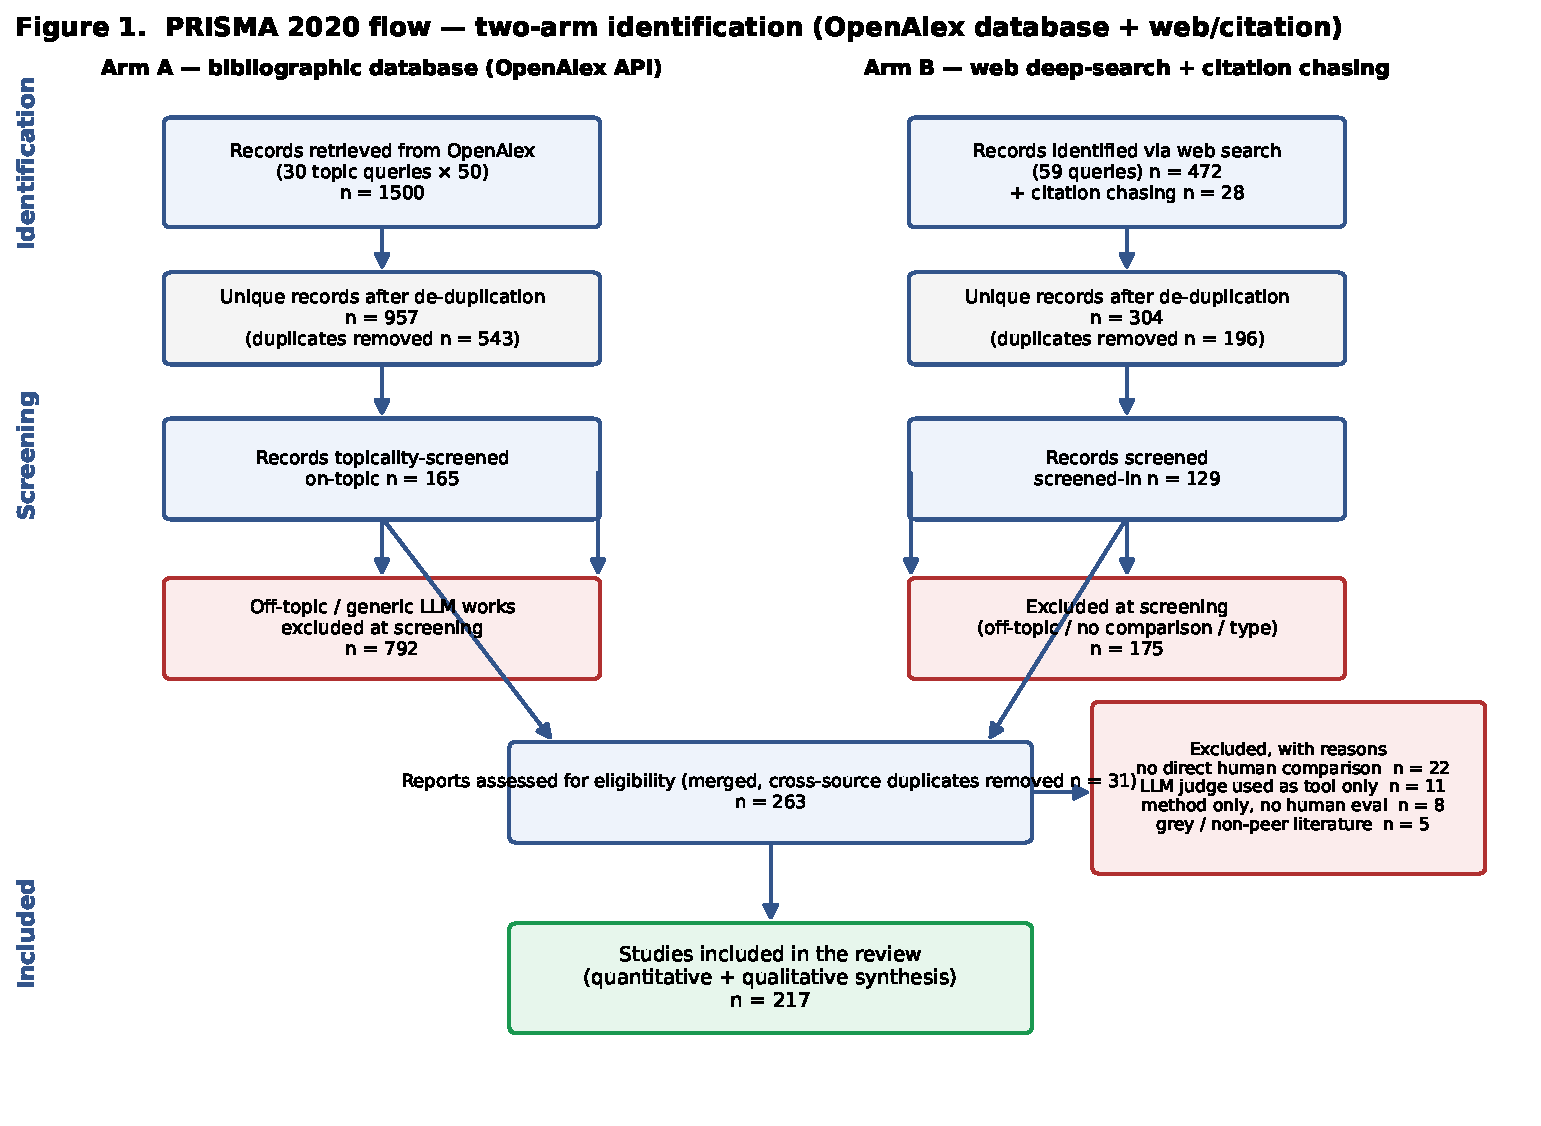
\includegraphics[width=0.96\linewidth]{fig01_prisma_flow}
\caption{Study 1 PRISMA~2020 flow (two-arm identification: OpenAlex database + web/citation).}
\label{fig:prisma1}
\end{figure}

\subsection{Findings: a green/amber/red landscape}
The modal verdict is \emph{mixed/task-dependent}; only \Pctreliable\% of studies sit in the reliable band and
\Pctproblematic\% in the problematic band (mean reliability \Meanrel/5). Reliability is governed by three properties:
\textbf{objectivity}, \textbf{tractable verification}, and a \textbf{low human-agreement floor}.
\textbf{Green ($\ge$3.5; \Ngreen{} domains):} machine translation (system level), text-to-image alignment,
verifiable instruction-following, QA/factuality, information extraction, general-NLG pairwise preference, dialogue,
and legal scoring: here LLM judges frequently match or exceed the human ceiling (e.g., MT-Bench 85\% vs.\ 81\%
human-human \citep{zheng2023mtbench}; GEMBA-MQM 96.5\% \citep{kocmi2023gembamqm}; SAFE wins 76\% of disagreements
\citep{wei2024safe}). \textbf{Amber (\Namber{} domains):} summarization, RAG, education, social-science annotation,
medicine (structure-dependent: $\kappa\!\approx\!0.82$-$0.93$ structured vs.\ $0.47$-$0.71$ complex reasoning),
code, and IR/relevance (strong but contested \citep{clarke2024cantreplace}). \textbf{Red (\Nred{} domains):}
low-resource multilingual evaluation and creative writing (near-zero expert correlation
\citep{chakrabarty2024artartifice}). Domain means over $n{\le}3$ studies (e.g.\ several single-study domains) are shown for completeness but flagged as low-confidence and should not be read to two-decimal precision; we rely on family-level aggregates for sparse cells. Figures~\ref{fig:dom1}-\ref{fig:land1} give the domain ordering and the
domain$\times$task landscape; the decision map (Figure~\ref{fig:dec1}) positions domains by reliability against
stakes.

\begin{figure}[t]\centering
\begin{subfigure}{0.5\linewidth}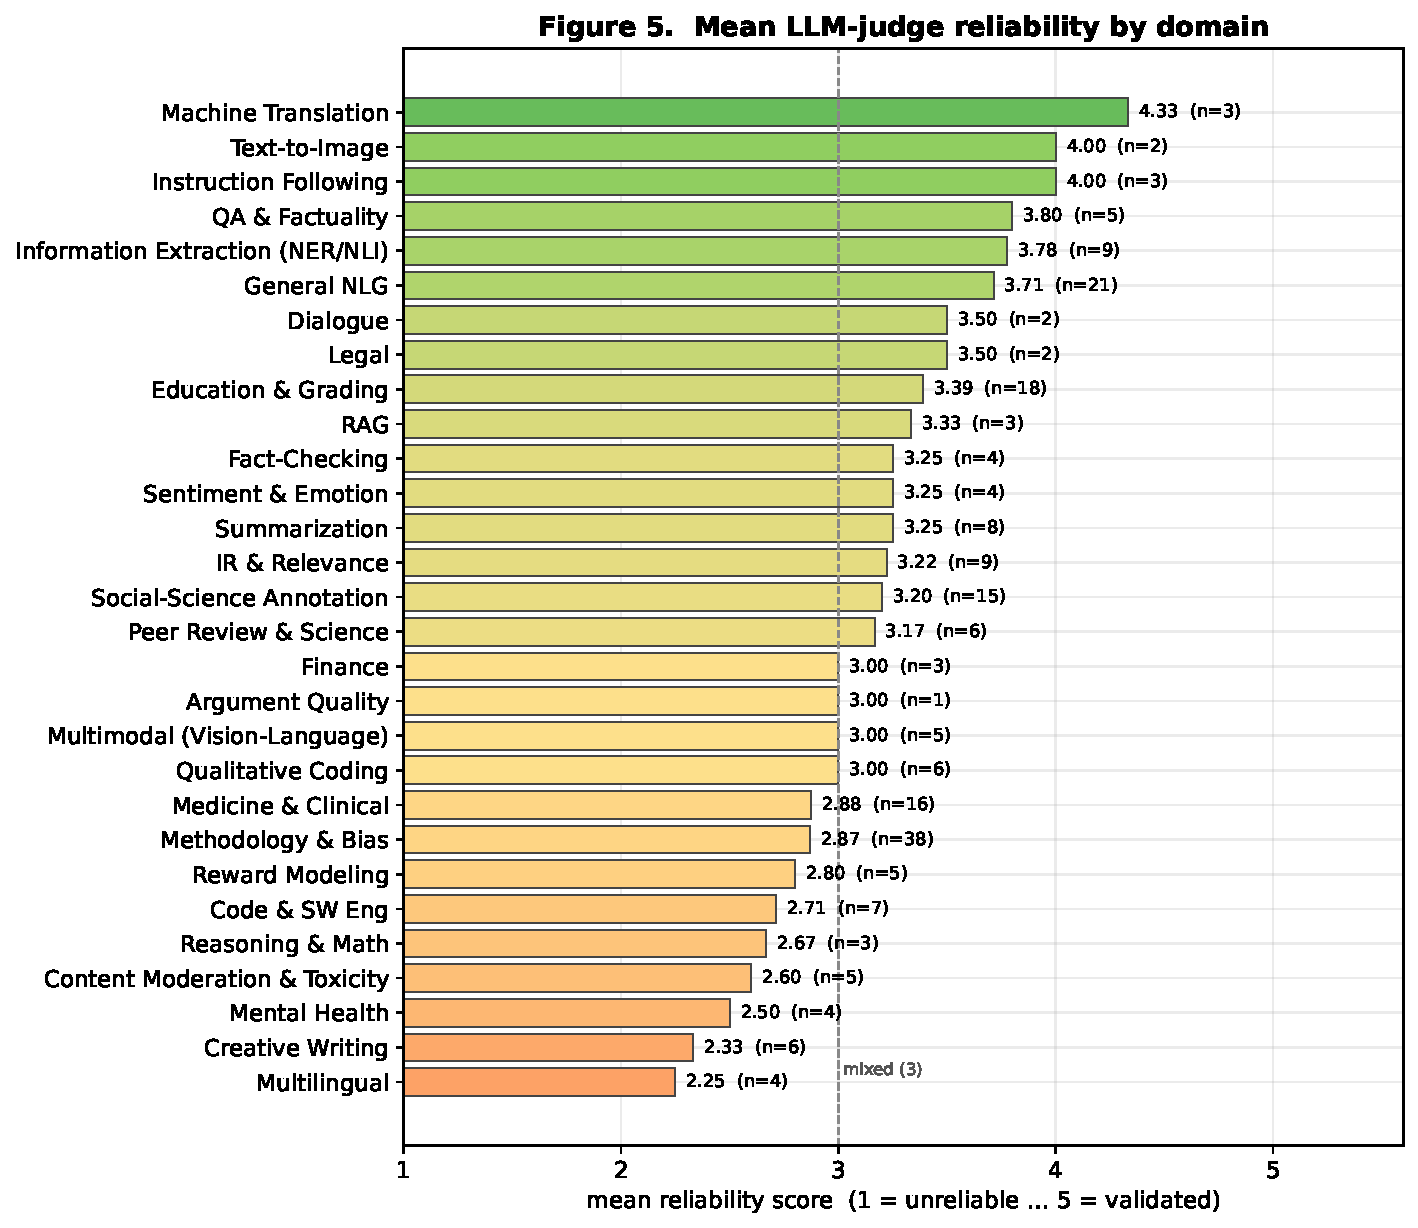
\includegraphics[width=\linewidth]{fig05_reliability_by_domain}\caption{}\label{fig:dom1}\end{subfigure}\hfill
\begin{subfigure}{0.48\linewidth}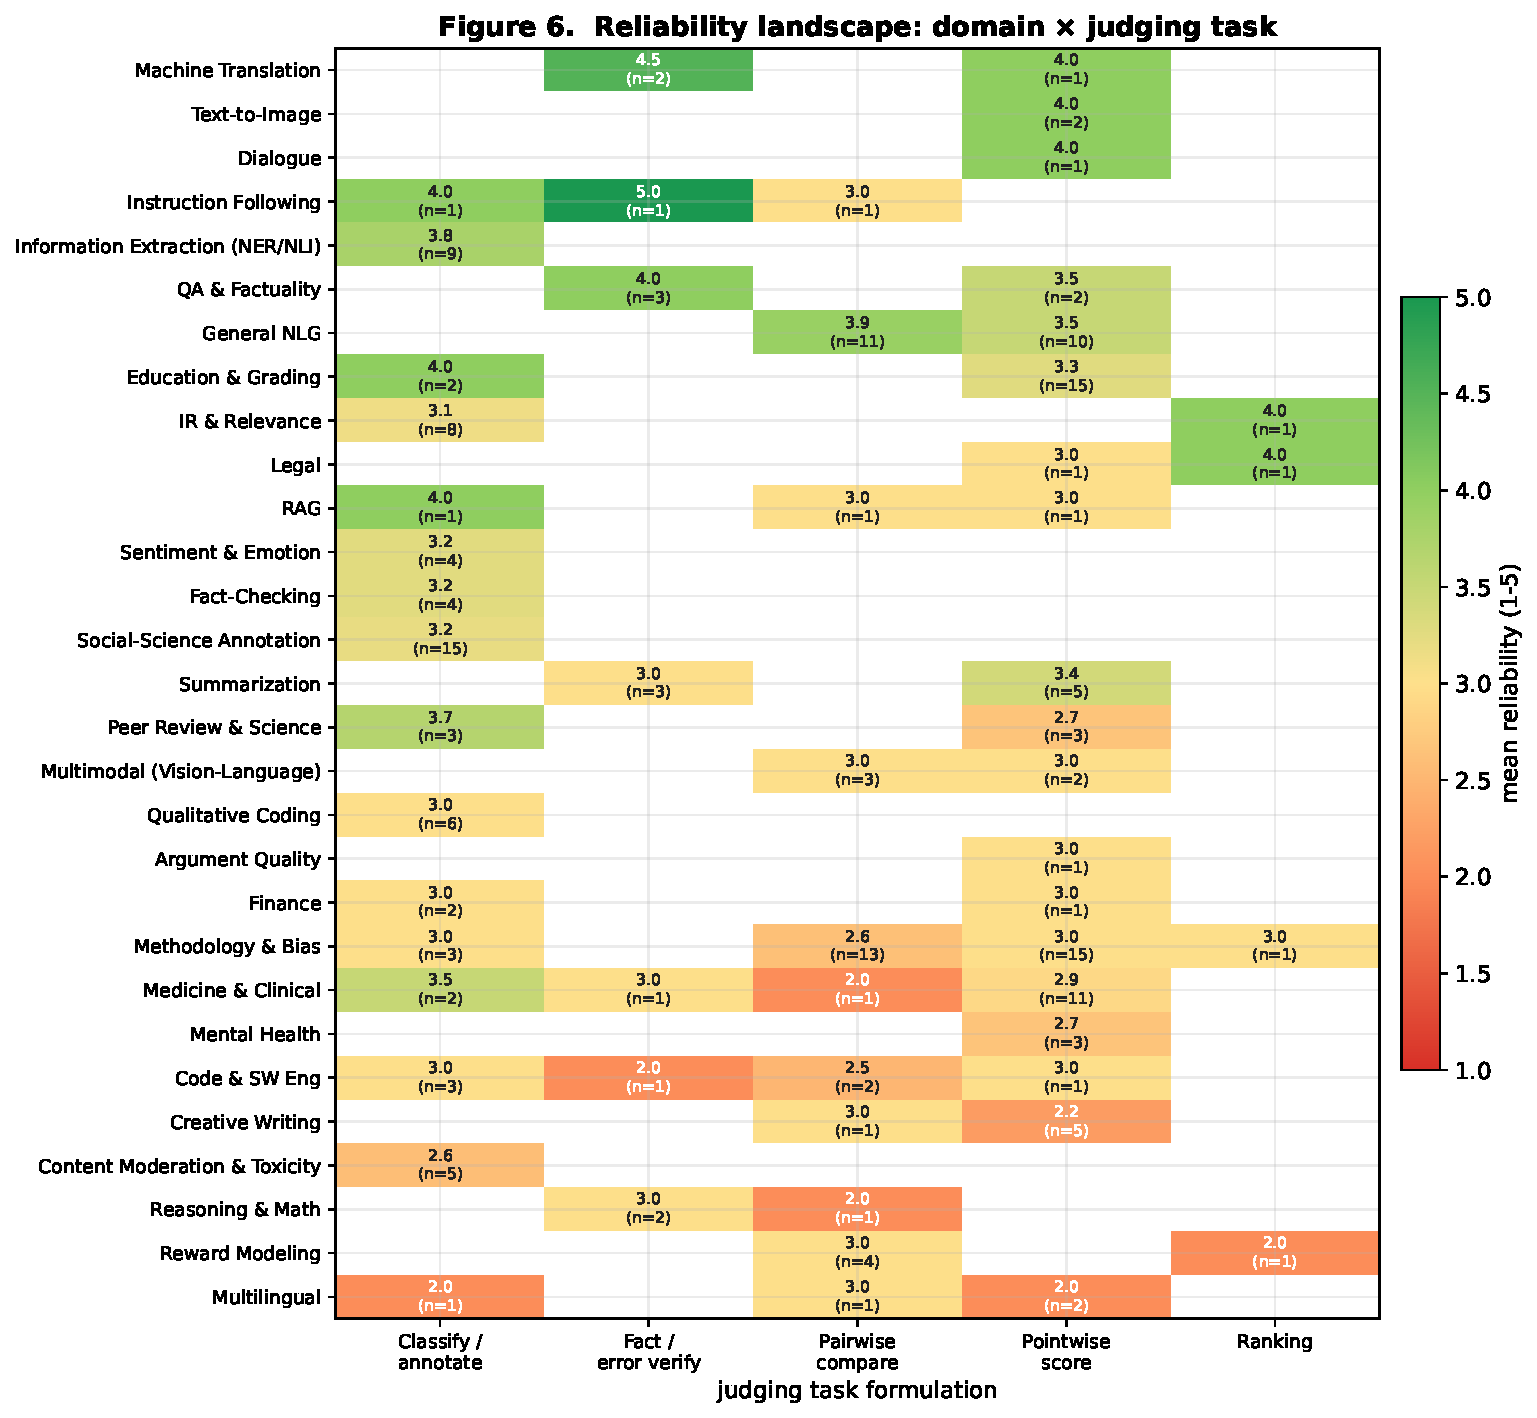
\includegraphics[width=\linewidth]{fig06_reliability_landscape}\caption{}\label{fig:land1}\end{subfigure}
\caption{Study 1. (a) Mean reliability by domain (green/amber/red). (b) Reliability landscape: domain$\times$judging
task; verification/classification columns are greener than open-ended scoring.}
\end{figure}

\subsection{Failure modes and the decision map}
Recurring biases such as verbosity/length, position, self-preference, style-over-substance, preference leakage,
non-determinism, and the \emph{expertise gap} (judges converge to crowd, not expert, consensus
\citep{bavaresco2024judgebench}) all modulate reliability (Figure~\ref{fig:bias1}). Agreement should be benchmarked
against the human ceiling, which on subjective tasks is itself low (Krippendorff $\alpha<0.35$
\citep{imrit2026iaa}). The Study-1a decision map (Figure~\ref{fig:dec1}) and Table~\ref{tab:decision} translate this into
deployment guidance and motivate the moving-target test (Study 2) that follows.

\begin{figure}[t]\centering
\begin{subfigure}{0.5\linewidth}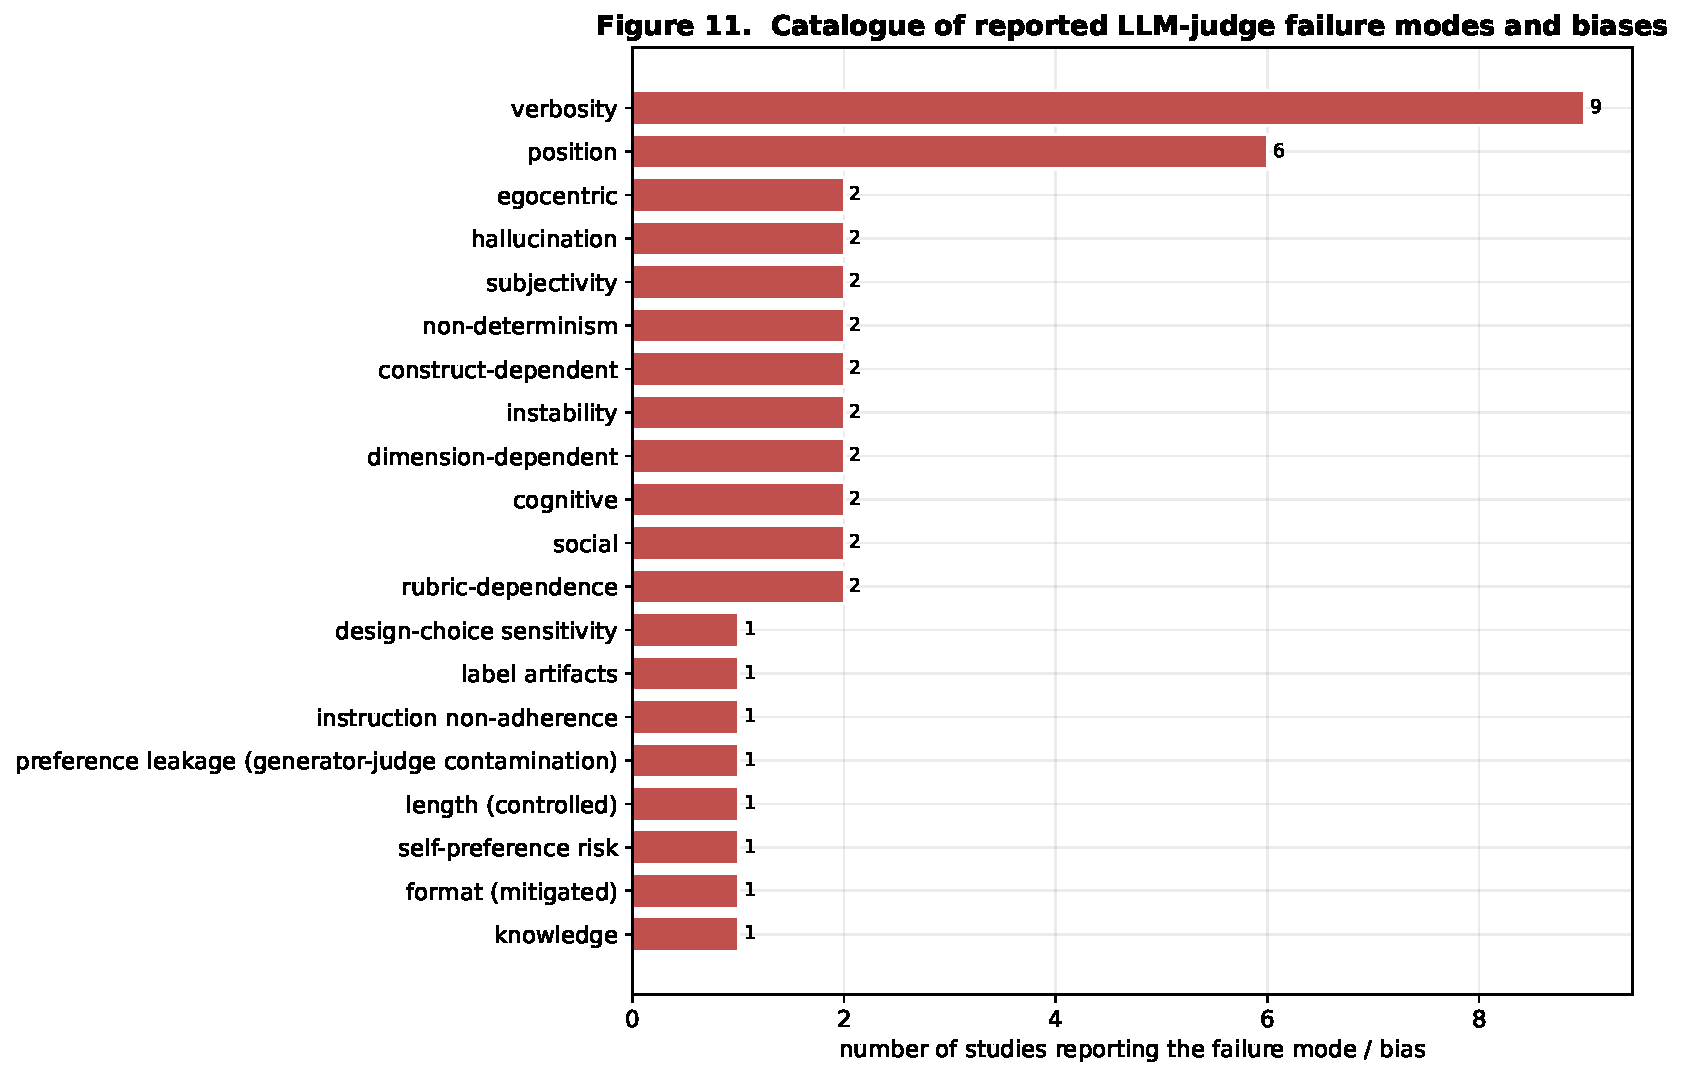
\includegraphics[width=\linewidth]{fig11_bias_frequency}\caption{}\label{fig:bias1}\end{subfigure}\hfill
\begin{subfigure}{0.49\linewidth}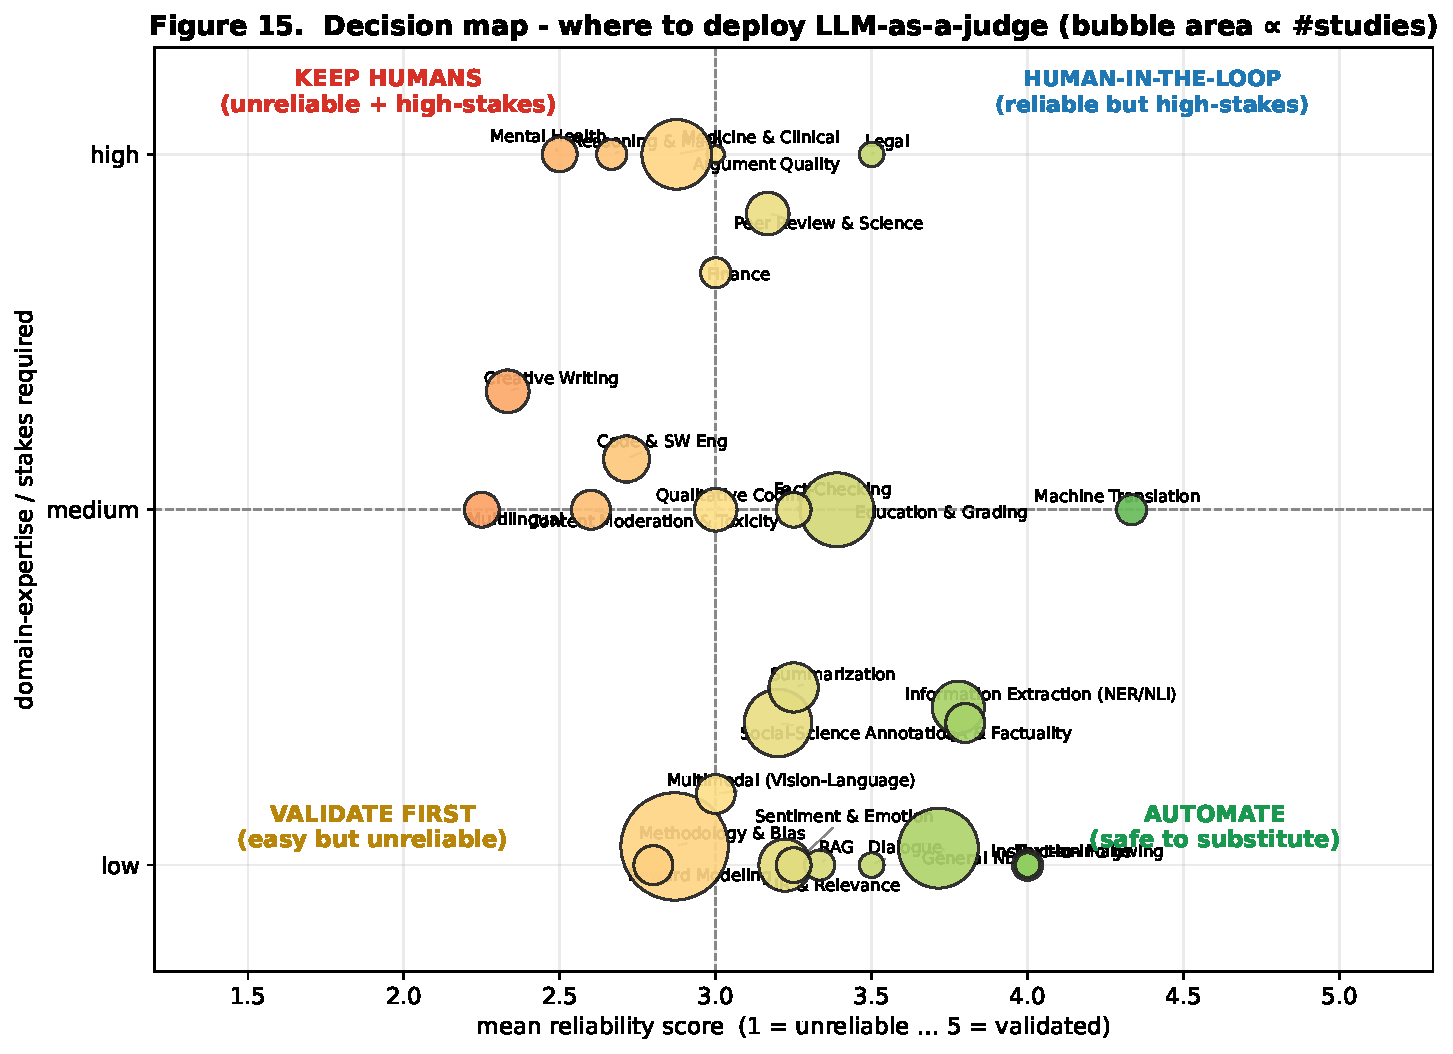
\includegraphics[width=\linewidth]{fig15_decision_map}\caption{}\label{fig:dec1}\end{subfigure}
\caption{Study 1. (a) Catalogue of reported failure modes/biases. (b) Deployment decision map (reliability$\times$
stakes; bubble area $\propto$ studies).}
\end{figure}

\begin{table}[tbp]\centering\small
\caption{Domain-level decision table. Mean reliability score (1 = unreliable $\dots$ 5 = validated), modal verdict,
and traffic-light signal (\textsc{green} $\ge 3.5$; \textsc{amber} 2.5-3.5; \textsc{red} $<2.5$). Sorted by mean
reliability. Small-$n$ domains should be read together with the family-level aggregates.}
\label{tab:decision}
\begin{tabular}{@{}l r c l c@{}}
\toprule
Domain / task & $n$ & Mean rel. & Modal verdict & Signal \\
\midrule
Machine Translation & 3 & 4.33 & Promising & \cellcolor{g!55}\textsc{green} \\
Text-to-Image & 2 & 4.00 & Promising & \cellcolor{g!55}\textsc{green} \\
Dialogue & 1 & 4.00 & Promising & \cellcolor{g!55}\textsc{green} \\
Instruction Following & 3 & 4.00 & Validated & \cellcolor{g!55}\textsc{green} \\
QA \& Factuality & 5 & 3.80 & Promising & \cellcolor{g!55}\textsc{green} \\
Information Extraction (NER/NLI) & 9 & 3.78 & Promising & \cellcolor{g!55}\textsc{green} \\
General NLG & 21 & 3.71 & Promising & \cellcolor{g!55}\textsc{green} \\
Legal & 2 & 3.50 & Promising & \cellcolor{g!55}\textsc{green} \\
Education \& Grading & 17 & 3.35 & Mixed & \cellcolor{a!60}\textsc{amber} \\
RAG & 3 & 3.33 & Mixed & \cellcolor{a!60}\textsc{amber} \\
Summarization & 8 & 3.25 & Promising & \cellcolor{a!60}\textsc{amber} \\
Fact-Checking & 4 & 3.25 & Promising & \cellcolor{a!60}\textsc{amber} \\
Sentiment \& Emotion & 4 & 3.25 & Mixed & \cellcolor{a!60}\textsc{amber} \\
IR \& Relevance & 9 & 3.22 & Promising & \cellcolor{a!60}\textsc{amber} \\
Social-Science Annotation & 15 & 3.20 & Mixed & \cellcolor{a!60}\textsc{amber} \\
Peer Review \& Science & 6 & 3.17 & Mixed & \cellcolor{a!60}\textsc{amber} \\
Multimodal (Vision-Language) & 5 & 3.00 & Mixed & \cellcolor{a!60}\textsc{amber} \\
Qualitative Coding & 6 & 3.00 & Mixed & \cellcolor{a!60}\textsc{amber} \\
Argument Quality & 1 & 3.00 & Mixed & \cellcolor{a!60}\textsc{amber} \\
Finance & 3 & 3.00 & Mixed & \cellcolor{a!60}\textsc{amber} \\
Medicine \& Clinical & 16 & 2.88 & Mixed & \cellcolor{a!60}\textsc{amber} \\
Methodology \& Bias & 38 & 2.87 & Mixed & \cellcolor{a!60}\textsc{amber} \\
Reward Modeling & 5 & 2.80 & Mixed & \cellcolor{a!60}\textsc{amber} \\
Code \& SW Eng & 7 & 2.71 & Mixed & \cellcolor{a!60}\textsc{amber} \\
Reasoning \& Math & 3 & 2.67 & Mixed & \cellcolor{a!60}\textsc{amber} \\
Content Moderation \& Toxicity & 5 & 2.60 & Mixed & \cellcolor{a!60}\textsc{amber} \\
Mental Health & 4 & 2.50 & Mixed & \cellcolor{a!60}\textsc{amber} \\
Creative Writing & 6 & 2.33 & Mixed & \cellcolor{r!55}\textsc{red} \\
Multilingual & 4 & 2.25 & Caution & \cellcolor{r!55}\textsc{red} \\
\bottomrule
\end{tabular}
\end{table}

% =====================================================================
\section{Study 2: Is the reliability landscape a moving target?}\label{sec:s1b}
% =====================================================================
A systematic review necessarily captures results \emph{as reported}, and most ``promising''-band evidence in
Study~1 was produced with proprietary judges that are now one or two model generations old (e.g.\ the influential
G-Eval used GPT-4). This raises a question that the review alone cannot answer: when an LLM judge falls short of the
human ceiling in a promising domain, is that a \emph{temporary} limitation that more capable models will erase
(``matter of time''), or a \emph{structural} property of LLM-as-a-judge that better models do not overcome? Study~2
answers this directly for a flagship case by re-running the evaluation with the most powerful open models available
to us today and comparing against the canonical reported numbers.

\subsection{Method}
We select \textbf{SummEval} \citep{fabbri2021summeval} (summarization quality assessment, a central amber-band task
in Study~1) because it pairs (i) a widely cited LLM-judge result to beat (G-Eval/GPT-4; \citealp{liu2023geval})
with (ii) public expert human ratings on four aspects (coherence, consistency, fluency, relevance) for
$100\times16=1600$ machine summaries. We replicate the G-Eval summary-level protocol \emph{verbatim} (same aspect
definitions, 1-5 integer ratings, temperature~0) but swap the judge for the \ONEmodels{} most powerful open models
in the available open-model catalogue (\ONEpanel). The comparison metric is the canonical \emph{summary-level Spearman}: for each
source document, correlate the judge's 16 scores with the human means, averaged across documents. The bar to beat is
G-Eval/GPT-4's reported per-aspect correlations (coherence~.582, consistency~.507, fluency~.455, relevance~.547;
average~$\approx$.52). In total Study~2 contributes \ONEnjudg{} fresh judgments.

\subsection{Results}
\begin{table}[t]\centering\small
\caption{Study 2. Summary-level Spearman $\rho$ of the most powerful open judges on SummEval vs.\ the reported
G-Eval-4/GPT-4 correlations (\ONEnjudg{} judgments). Green cells \emph{surpass} the reported per-aspect number.}
\label{tab:study1b}
\begin{tabular}{@{}l cccc c@{}}
\toprule
Judge & Coher. & Consist. & Fluency & Relev. & Avg $\rho$ \\
\midrule
\textit{Reported (G-Eval-4)} & 0.582 & 0.507 & 0.455 & 0.547 & 0.523 \\
\midrule
\texttt{deepseek-v4-pro} & 0.548 & \cellcolor{g!30}0.688 & 0.392 & 0.540 & \cellcolor{g!30}0.542 \\
\texttt{qwen3.6-35b-a3b} & \cellcolor{g!30}0.606 & \cellcolor{g!30}0.702 & 0.298 & 0.540 & \cellcolor{g!30}0.536 \\
\texttt{glm-5.1} & \cellcolor{g!30}0.650 & \cellcolor{g!30}0.693 & 0.217 & 0.543 & \cellcolor{g!30}0.526 \\
\texttt{gptoss-120b} & \cellcolor{g!30}0.586 & \cellcolor{g!30}0.685 & 0.260 & 0.482 & 0.503 \\
\bottomrule
\end{tabular}
\end{table}
We follow the standard summary-level G-Eval protocol \citep{liu2023geval} and attach bootstrap 95\% CIs (over the
100 source documents) to every correlation (Figure~\ref{fig:s1b}, Table~\ref{tab:study1b}). On the verifiable
aspects the open judges \emph{meet or exceed} the established G-Eval/GPT-4 benchmark: \RTwobeats{} of the 16
model$\times$aspect cells have a 95\% CI lying \emph{entirely above} the reported value, all on \textbf{consistency}
and \textbf{coherence} (e.g.\ \ONEbest{} consistency $\rho{=}0.69$, CI $[0.63,0.74]$ vs.\ $.507$), and
\textbf{relevance} is on par ($.48$-$.54$ vs.\ $.55$). \textbf{Controlling for the scoring protocol.} A natural
concern is that G-Eval's reported numbers use \emph{probability-weighted} token decoding whereas we read a single
integer, so the difference could be a scoring artifact rather than a model effect. We test this directly: for a model
that emits a clean score-token distribution (gemma-4-31b) we recompute summary-level Spearman under both an integer
(argmax) score and G-Eval's probability-weighted expected score, from the same calls. The two agree closely
(coherence $\PWintCoh$/$\PWexpCoh$, fluency $\PWintFlu$/$\PWexpFlu$, relevance on par); consistency is the one
aspect where the two diverge ($\PWintCon$ integer vs $\PWexpCon$ probability-weighted), but both remain at or above
the reported $.507$. The open-model result is therefore not an artifact of integer scoring, and the comparison to the
reported benchmark is fair on this axis. But on \textbf{fluency} every open model falls well
\emph{short} ($.22$-$.39$ vs.\ a reported $.455$). We diagnose why: fluency is the most \emph{compressed} aspect of
the human reference, with the lowest within-document rating variance ($\mathrm{SD}=\SEfluSD$ vs $\SEconSD$ for
consistency) and $\SEfluTop\%$ of summaries rated near the top of the scale, so it offers the least to rank, and it
is the aspect on which the \emph{reported proprietary judge also scores lowest}. This is a property of the
\emph{reference}, not the judges: even a noiseless judge returning the rounded human means tops out at
$\rho{\approx}\SEfluSelf$ on fluency. The clean result is therefore that capability gains concentrate on the
verifiable, rankable aspects (consistency, coherence), while the most compressed aspect is hard to rank for every
judge, open or proprietary.

\begin{figure}[t]\centering
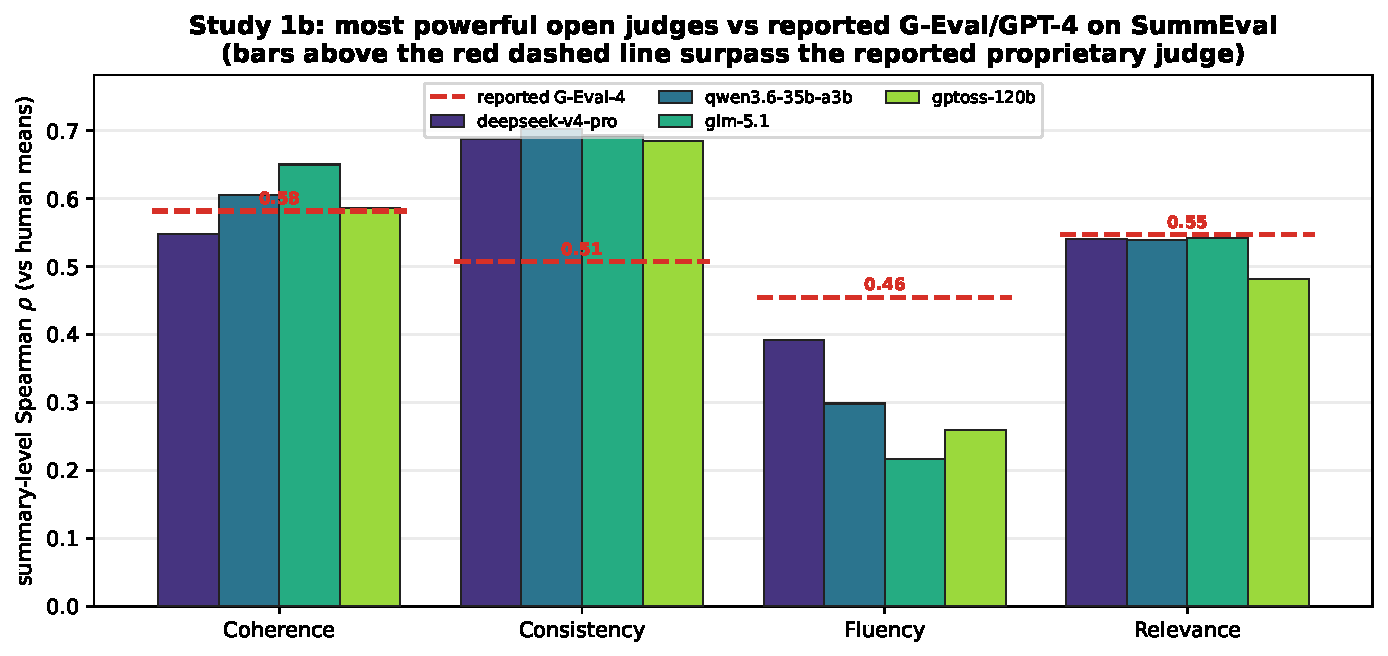
\includegraphics[width=0.97\linewidth]{s1b_fig01_spearman}
\caption{Study 2. Summary-level Spearman of the most powerful open judges on SummEval, per aspect, against the
reported G-Eval/GPT-4 bar (dashed). Bars above the dashed line indicate an open model that \emph{surpasses} the
reported proprietary-judge correlation.}
\label{fig:s1b}
\end{figure}

\paragraph{Interpretation: time vs.\ structure.} Study~2 shows the reliability landscape is \emph{partly} a moving
target. Where Study~1's amber rating reflected a capability gap on a verifiable sub-judgment, today's open models
close or exceed it; reliability there is largely a matter of time and access. But where the shortfall reflects a
\emph{compressed or contested human ceiling} (e.g.\ fluency, and, as Study~3 will show, subjective social annotation),
even the most powerful models do not break through, because the limit lives in the human reference, not the model.
This distinction, temporal capability gap vs.\ structural ceiling, is the lens we carry into HCC.

\paragraph{Takeaway.} Study~1 says LLM judges are safe where the task is objective and verifiable, and
Study~2 shows that frontier open models are now strong enough to match proprietary judges on exactly those
verifiable tasks. But subjective, high-disagreement constructs (the kind that
humans themselves contest) are precisely the tasks Study~1 flags as risky and Study~2
predicts scale will \emph{not} fix. Study~3 then tests this prediction directly, on datasets with rich human label distributions.

% =====================================================================
% =====================================================================
\section{Study 3: An open-panel meta-evaluation on NLI with rich human labels}\label{sec:study3}
% =====================================================================
Study 1 shows LLM judges are most reliable where the human-agreement ceiling is high and verifiable; Study 2 shows
frontier open models reach the established benchmark on the verifiable aspects of summarization. Study 3 tests the
mechanism directly on \emph{natural language inference} (NLI), the rare setting that ships \emph{rich} human label
distributions: ChaosNLI \citep{plank2022humanlabel} re-annotates SNLI and MultiNLI items with ${\sim}100$ human
labels each, so the human-human agreement ceiling and the per-item disagreement are measured precisely rather than
estimated from three annotators.

\subsection{Method}
We evaluate a panel of \STHRmodels{} open models served via \PROVIDER{} (OpenAI-compatible), spanning five families
and 9B-754B parameters, run at temperature~0. Each model labels every item as a virtual annotator under the
standard NLI instructions; we benchmark against the \emph{human-human ceiling} (random-annotator-vs-majority
accuracy with an annotator bootstrap 95\% CI, plus pairwise agreement), and report accuracy, Cohen's $\kappa$, and
macro-F1 against the majority gold, a majority \textbf{jury} \citep{verga2024poll}, and a calibrated
contamination screen. The run comprised \NLInjudg{} judgments across \NLIndat{} NLI datasets with zero API errors
and a 100\% answer-parse rate. Dataset cards, prompts, and metric definitions are in
Appendices~\ref{app:protocol} to~\ref{app:robust}.

\subsection{Results}
Table~\ref{tab:nlires} reports the panel against the human ceiling. Where humans agree only moderately
(SNLI ceiling 0.75, MNLI 0.64), the open panel \emph{matches or exceeds} a single held-out human: on SNLI 5/6 models
reach the human-human ceiling (we mark this \textbf{Validated}, but treat the verdict as \emph{conditional}, since
SNLI/MultiNLI are old corpora and we cannot exclude memorization; see below), with MNLI \textbf{Promising}.
Chance-corrected agreement is substantial (best-model $\kappa$ up to 0.71). The jury reaches 0.86 ($>$ the 0.75
single-annotator ceiling), but we caution that a six-model aggregate exceeding a \emph{single}-held-out-human ceiling
is expected and does not imply super-human reliability; we report it as panel stability, not a ceiling-breaking
result.

\begin{table}[t]\centering\small
\caption{Study 3 (NLI). Open panel vs the human-human ceiling. Ceiling = random-annotator-vs-majority accuracy;
macro-F1 is the best model's chance-corrected score.}
\label{tab:nlires}
\begin{tabular}{@{}l l c c c c l@{}}
\toprule
Dataset & Construct & Human & Best model & macro-F1 & Jury & Modal verdict \\
 & & ceiling & (acc) & (best) & (acc) & \\
\midrule
ChaosNLI-SNLI & NLI (3-way) & 0.75 & 0.84 (gemma-4-31b) & 0.79 & 0.86 & \cellcolor{g!55}Validated \\
ChaosNLI-MNLI & NLI (3-way) & 0.64 & 0.70 (gemma-4-31b) & 0.70 & 0.65 & \cellcolor{g!25}Promising \\
\bottomrule
\end{tabular}
\end{table}

\subsection{Judges track the human ceiling across the disagreement spectrum}
Panel accuracy declines on high-human-disagreement (high-entropy) items ($\NLIaccLowE$ on low-entropy vs
$\NLIaccHighE$ on high-entropy; Table~\ref{tab:nlidis}), but this is not a judge deficiency: the human ceiling
declines in lockstep, so the \emph{judge-vs-ceiling gap} is essentially zero at both ends ($\NLIgapLow$ on
low-entropy, $\NLIgapHigh$ on high-entropy items). In other words, open judges are at human level on NLI regardless
of how much humans disagree; the accuracy curve simply follows the ceiling. What residual variance there is lives at
the item level: in an item-level GLMM the random-intercept SD across \emph{items} ($\mathrm{SD}_{\text{logit}}=
\NLIitemSDlogit$) far exceeds that across \emph{models} ($\mathrm{SD}_{\text{logit}}=\NLImodelSDlogit$, on the same
logit scale), and standardized model scale contributes modestly ($\mathrm{OR}_{/\mathrm{SD}}=\RTwosizeOR$). We do
not fit a dataset-level model (two datasets cannot support one). \emph{Contamination caveat:} SNLI and MultiNLI are
older public corpora, and our verbatim-recall screen false-positives on high-recall models even for guaranteed-clean
text (Appendix~\ref{app:robust}); we therefore cannot rule out that some of the NLI agreement reflects memorization,
and we report this as a genuine threat to the ``Validated'' verdict that a post-cutoff NLI benchmark would resolve.
Juries raise accuracy but cannot lift agreement above the human ceiling.

\begin{table}[t]\centering\small
\caption{Study 3 (NLI) disagreement-aware results. Ceiling with annotator-bootstrap 95\% CI; best-model $\kappa$ and
macro-F1; panel accuracy on low- vs high-human-disagreement items; Jensen-Shannon panel-vs-human divergence.}
\label{tab:nlidis}
\begin{tabular}{@{}l c c c c c c@{}}
\toprule
Dataset & Ceiling [95\% CI] & $\kappa$ & macro-F1 & acc$_{\downarrow H}$ & acc$_{\uparrow H}$ & JS \\
 & & (best) & (best) & low-disagr. & high-disagr. & \\
\midrule
ChaosNLI-SNLI & 0.75 [0.74,0.77] & 0.71 & 0.79 & 0.89 & 0.67 & 0.09 \\
ChaosNLI-MNLI & 0.64 [0.63,0.65] & 0.53 & 0.70 & 0.68 & 0.55 & 0.17 \\
\bottomrule
\end{tabular}
\end{table}
% =====================================================================
\section{Discussion}
% =====================================================================
\subsection{What governs LLM-judge reliability}
Across the three studies one principle organizes the evidence: an LLM judge is reliable to the degree that the task
has a high, verifiable human-agreement ceiling, and it cannot exceed an agreement level that humans themselves do
not reach. Study~3 localizes the mechanism at the \emph{item} level: on the same logit scale the random-intercept SD
of judge correctness is far larger across items ($\mathrm{SD}_{\text{logit}}=\NLIitemSDlogit$) than across models
($\NLImodelSDlogit$), and the judge-vs-ceiling gap is near zero across the human-disagreement spectrum, so open
judges are at human level on NLI regardless of how much humans disagree. Model scale helps only modestly
($\mathrm{OR}_{/\mathrm{SD}}=\RTwosizeOR$). We are careful about the unit of analysis: with two NLI datasets we do
not fit a dataset-level model. We also do not claim contamination is excluded; SNLI/MultiNLI are old corpora and our
recall screen is only a conservative check (Appendix~\ref{app:robust}), so memorization remains a live alternative
that a post-cutoff NLI benchmark would adjudicate.

\subsection{Connection to measurement and disagreement scholarship}
This result operationalizes a long-running argument that there is no single ground truth for subjective constructs
\citep{aroyo2015truth,plank2022humanlabel}: when judges are benchmarked against the human-human ceiling rather than a
forced majority, their ``failures'' on contested items are revealed as properties of the construct's contested human reference, not fixable model deficits. Reporting a single accuracy against a majority gold imposes
consensus where the data shows disagreement; the honest object of evaluation is the human label \emph{distribution}.

\subsection{Implications for designing LLM-as-a-judge experiments}
The evidence yields a concrete, reusable protocol. Any study using an LLM-as-a-judge should:
\begin{enumerate}[leftmargin=1.5em,itemsep=2pt]
\item \textbf{Anchor to the human-human ceiling}, not a single gold; report the ceiling (computed from the annotator
distribution at the dataset's native annotator count) and the judge-vs-ceiling gap.
\item \textbf{Match the metric to the construct}: on imbalanced tasks report macro-F1 and per-class scores and
prefer disagreement-aware evaluation against the full label distribution over forced-majority accuracy.
\item \textbf{Quantify uncertainty}: bootstrap confidence intervals for every comparison; do not assert ``beats/
matches'' from point estimates.
\item \textbf{Stratify by item difficulty}: because variance lives in items, report where the judge fails (high
human-disagreement items), not only mean accuracy.
\item \textbf{Probe contamination, but calibrate the probe}: evaluate on post-cutoff data where possible, and treat
surface-recall probes as conservative screens (they false-positive on high-recall models).
\item \textbf{Pin the setup}: fix model identifier, version, decoding (temperature, seed); report robustness to
prompt paraphrase, since small models are prompt-sensitive on subjective tasks.
\item \textbf{Use juries for aggregate decisions} but not as a ceiling-breaker: panels improve stability yet do not
lift a subjective task above its human ceiling.
\item \textbf{Pre-register and release}: register the construct, the human baseline, and the decision threshold, and
release item-level labels and aggregates.
\end{enumerate}

\subsection{A decision framework}
For annotation and evaluation tasks, three regimes follow from the human-ceiling principle. \textbf{Automate (with
light audit):} objective, verifiable judgments (entailment, factual consistency, instruction-following) where the
human ceiling is high, exactly where Study~3's NLI panel reaches or exceeds it. \textbf{Calibrate and audit:}
judgments with a low or moderate ceiling, where a judge can post high accuracy by predicting base rates, so report
chance-corrected agreement ($\kappa$) and audit the high-disagreement items. \textbf{Keep humans in the loop:}
constructs on which human annotators themselves disagree sharply, where no open judge can exceed a ceiling humans do
not reach. A critical caution for the field: agreement on older public benchmarks can reflect memorization
\citep{bender2021parrots}, and a single headline accuracy can mask base-rate learning, so calibrated,
disagreement-aware, post-cutoff evaluation should be the norm. The application of these ideas to the subjective,
interpretive tasks of Human-Centered Computing is the subject of a companion paper.
% =====================================================================
\section{Limitations}
% =====================================================================
The \emph{human} validation here is inherited from prior work, not added by us: Study 3's ground truth is ChaosNLI's
${\sim}100$ human labels per item, and the Study 1 review codes each study against the human baselines those studies
report. The review verdict is our interpretation (only \Nnumeric{} of \Nstudies{} report an extractable numeric
agreement value); we report an independent re-coding as a reproducibility check (Krippendorff $\alpha=\IRRsoneA$,
$100\%$ within one level; Appendix~\ref{app:irr}), which is LLM-assisted and therefore measures rubric
reproducibility. All \Nstudies{}${+}\STN{}$ references were web-verified and two unverifiable entries removed.
By design we evaluate \emph{open} models (the reproducible choice for most researchers) at temperature~0; Study 2
uses one summarization benchmark with integer scoring, and Study 3's deep human-label data are available for NLI
rather than every domain. Subjective social-computing annotation, where the human ceiling is contested, is the focus
of a companion paper. The six-model panel spans five families but shares overlapping pretraining lineages, so the between-model variance
is a lower bound on judge diversity. Findings reflect models available through mid-2026.
\section{Ethics and reproducibility}
% =====================================================================
\textbf{Ethics.} The review analyzes published research, not human subjects, and Study 3 reuses already-public,
de-identified NLI datasets under their licenses; this work was therefore not human-subjects research requiring IRB
review, and we sought an exemption determination consistent with our institution's policy. We release only
item-level labels and aggregate statistics. One ethical point bears on the method itself: treating the
\emph{majority} human label as ``ground truth'' for the ceiling can encode majority bias and erase minority readings,
which is why we report the full disagreement (soft labels, entropy) rather than only the majority and recommend
disagreement-aware evaluation. The contamination screen is reported precisely so ``validated'' verdicts are not
silently inflated by pretraining exposure.
\textbf{Reproducibility.} Every number in this paper regenerates from released code: the OpenAlex, Semantic Scholar,
and web search logs; the coded corpus; the figure and table generators; the SummEval harness and the
Study-3 judging/scoring/contamination/mixed-effects harness, all keyed to documented model identifiers served through
\PROVIDER{} at temperature~$0$ with idempotent, resumable checkpoints. The auto-generated statistics macros
mean the manuscript cannot drift from the data. Repository: \REPO{}.

% =====================================================================
% =====================================================================
\section{Conclusion}
% =====================================================================
Open, locally-servable LLMs are now strong enough to serve as judges on objective, verifiable tasks: on the
verifiable aspects of a summarization benchmark they meet or exceed the reported proprietary-judge correlations, and
on NLI they reach the human-human ceiling (a conditional verdict, given possible contamination of these older corpora). But across \Nstudies{} reviewed studies and a
\NLInjudg{}-judgment meta-evaluation on NLI datasets with rich human labels, reliability is bounded by the same thing
for every model: the \emph{human-human agreement ceiling}, and it degrades on exactly the items where humans
themselves disagree. Scaling the judge helps only modestly; contamination cannot be excluded on these older NLI corpora and is stated as a limitation. The
practical consequence is that an LLM-as-a-judge should be reported the way we report any measurement instrument,
against a human reference, with chance-corrected and disagreement-aware metrics, with uncertainty, and with a stated
operating range, rather than trusted as an oracle. The right question is never ``can a machine judge?'' but ``can
this open model agree with humans, on this construct, as well as humans agree with each other?''

\bibliographystyle{ACM-Reference-Format}
\bibliography{references}
\appendix

% =====================================================================
\section{Review protocol and reliability rubric}\label{app:protocol}
% =====================================================================
\paragraph{Identification.} The review follows PRISMA~2020. The primary bibliographic source is the \textbf{OpenAlex} API; we cross-check with the \textbf{Semantic Scholar} Graph API and a structured \textbf{web ``deep-research''} arm (a 59-query protocol plus venue-scoped sweeps). Concept blocks combine an LLM term (``LLM'', ``large language model'', ``GPT-4'', ``ChatGPT'', ``Gemini'') with an evaluation/agreement term (``LLM-as-a-judge'', ``automatic evaluation'', ``annotation'', ``inter-annotator agreement'', ``human evaluation''). Records were deduplicated by DOI and normalized title.

\paragraph{Screening and eligibility.} \emph{Inclusion:} peer-reviewed or preprint studies that empirically compare
LLM judgments to human judgments on the same items and report (or allow computing) an agreement statistic.
\emph{Exclusion:} non-empirical position papers, studies with no human baseline, studies that use LLMs only to
generate (not judge) content, and off-topic retrievals. Title/abstract screening was followed by full-text
eligibility assessment; per-stage counts appear in the PRISMA flow figures (Figure~\ref{fig:prisma1}).

\paragraph{Reliability verdict (five-level rubric).} Each study is coded against the \emph{human-human agreement
ceiling} for its task:
\begin{itemize}[leftmargin=1.4em,itemsep=1pt]
\item \textbf{1 Validated:} LLM-human agreement is at or above the human-human ceiling (substitution is empirically
justified).
\item \textbf{2 Promising:} agreement approaches the ceiling under specific, reported conditions (model, prompt,
aggregation); conditional substitution.
\item \textbf{3 Mixed:} results are task- or setup-dependent and inconsistent across studies.
\item \textbf{4 Caution:} agreement is consistently and materially below the ceiling.
\item \textbf{5 Unreliable:} agreement is near chance or dominated by bias (position, verbosity, self-preference).
\end{itemize}
We report a reliability score $=6-\text{verdict}$ and synthesize within metric families (e.g.\ Cohen's $\kappa$,
Krippendorff's $\alpha$, Spearman $\rho$, accuracy) rather than pooling incommensurable effect sizes. The full coded corpus (Appendix~\ref{app:s1}) is released for re-coding.

% =====================================================================
\section{Study 2: G-Eval replication details}\label{app:s1bdetail}
% =====================================================================
We replicate the summary-level G-Eval protocol \citep{liu2023geval} on SummEval \citep{fabbri2021summeval}
($100$ source articles $\times$ $16$ system summaries $=1600$ summaries, each with expert means for four aspects).
Each (summary, aspect) pair is scored $1$ to $5$ by the judge with the aspect criterion below; we then compute the
\textbf{summary-level Spearman} $\rho$ (per source document, correlate the judge's $16$ scores with the human means,
averaged over documents, dropping documents with no score variance) and compare it to the reported G-Eval-4/GPT-4
correlations. Judges are the four most powerful open models in the available open-model catalogue
(\texttt{glm-5.1-fp8}~$754$B, \texttt{deepseek-v4-pro}, \texttt{gptoss-120b}, \texttt{qwen3.6-35b-a3b-fp8}), decoded
at temperature~$0$. Aspect criteria (verbatim):
\begin{quote}\small
\textbf{Coherence (1-5):} the collective quality of all sentences; the summary should be well-structured and
well-organized, building from sentence to sentence into a coherent body of information, not just a heap of related
information.\\[2pt]
\textbf{Consistency (1-5):} factual alignment between the summary and the source; a consistent summary contains only
statements entailed by the source document; hallucinated or unsupported facts are penalized.\\[2pt]
\textbf{Fluency (1-5):} the quality of individual sentences (grammar, capitalization, readability).\\[2pt]
\textbf{Relevance (1-5):} selection of the most important content from the source; redundancy and unimportant
content are penalized.
\end{quote}
The judge receives the source article and the summary and returns only a JSON object \verb|{"score": <1-5>}| (a
larger token budget and a retry handle reasoning-model outputs). In total Study~1b contributes \ONEnjudg{} judgments.

% =====================================================================
\section{Study 3: datasets, judging prompts, and metrics}\label{app:s3detail}
% =====================================================================
\paragraph{Datasets.} Study 3 uses the \NLIndat{} ChaosNLI datasets (Table~\ref{tab:cardsnli}); each is sampled to
$n{=}500$ items with a clear majority label (ties dropped), and the ${\sim}100$ human labels per item give a precise
human ceiling.

\begin{table}[h]\centering\small
\caption{Study 3 (NLI) dataset cards. Ceiling $=$ random-annotator-vs-majority accuracy.}
\label{tab:cardsnli}
\begin{tabular}{@{}l l l c c@{}}
\toprule
Dataset & Task & Source & Annot./item & Ceiling \\
\midrule
ChaosNLI-SNLI & NLI (3-way) & SNLI + ChaosNLI relabels & ${\sim}100$ & 0.75 \\
ChaosNLI-MNLI & NLI (3-way) & MultiNLI + ChaosNLI relabels & ${\sim}100$ & 0.64 \\
\bottomrule
\end{tabular}

\end{table}

\paragraph{Models.} Table~\ref{tab:modelsA} lists the judge panel. Anonymized identifiers map to open-weight families; exact checkpoint identifiers, revisions, and quantization are released in the non-anonymous version.
\begin{table}[h]\centering\small
\caption{Judge panel (Studies 2--3).}\label{tab:modelsA}
\begin{tabular}{@{}l l r l@{}}
\toprule
Model (anonymized id) & Family & Params & Serving \\
\midrule
\texttt{qwen3.5-9b} & Qwen (Alibaba) & 9B & vLLM, bf16 \\
\texttt{qwen3.6-27b-fp8} & Qwen (Alibaba) & 27B & vLLM, fp8 \\
\texttt{gemma-4-31b} & Gemma (Google) & 31B & vLLM, bf16 \\
\texttt{gptoss-120b} & GPT-OSS (open) & 120B & vLLM, bf16 \\
\texttt{deepseek-v4-pro} & DeepSeek (MoE) & ${\sim}671$B & vLLM, fp8 \\
\texttt{glm-5.1-fp8} & GLM (open) & 754B & vLLM, fp8 \\
\bottomrule
\end{tabular}

\end{table}

\paragraph{Judging prompt.} Each model labels every item as a virtual annotator, returning a JSON label on the final
line (parsed with a surface-form-to-code map):
\begin{quote}\small\ttfamily
Premise: \{premise\} / Hypothesis: \{hypothesis\} / Does the premise ENTAIL the hypothesis, CONTRADICT it, or is it
NEUTRAL? -> \{"label": "entailment"|"neutral"|"contradiction"\}
\end{quote}

\paragraph{Metrics.} Let an item have $A$ human annotations with majority label $y^\star$. \textbf{Human ceiling} is
the random-annotator-vs-majority accuracy (expected agreement of one held-out human with the majority), averaged over
items; we also report pairwise human agreement, and bootstrap its 95\% CI by resampling annotators within items.
\textbf{Accuracy}, \textbf{Cohen's $\kappa$}, and \textbf{macro-F1} are against $y^\star$; the \textbf{jury} is the
per-item panel majority \citep{verga2024poll}; \textbf{95\% CIs} are nonparametric bootstrap (1000 item resamples).
\textbf{Contamination screen:} the judge is given the dataset name and a one-third prefix of an item and asked to
reproduce the remainder; we report mean normalized overlap, but a clean-control (Appendix~\ref{app:robust}) shows it
false-positives on high-recall models, so we treat it as a conservative screen. The run recorded \emph{zero} API
errors and a 100\% answer-parse rate across all \NLInjudg{} judgments.

\paragraph{Inferential model.} We model each judgment's correctness ($\mathbf{1}[\text{judge}=y^\star]$) with an
item-level Bayesian logistic GLMM with random intercepts for item and model, and report the variance components on a
common logit scale (item $\mathrm{SD}_{\text{logit}}=\NLIitemSDlogit$, model $\NLImodelSDlogit$). With two datasets
we do not fit a dataset-level model. To test whether the accuracy decline on high-disagreement items is a label-noise
artifact, we bin items by human entropy and report the judge-vs-ceiling \emph{gap} per bin (it is near zero
throughout for NLI, see the main text).

% =====================================================================
\section{Inter-coder reliability}\label{app:irr}
% =====================================================================
Because the reliability verdict and the role/stance codes embed judgement, we re-coded a held-out random sample of
each corpus with two \emph{independent} coders who saw only the per-study summaries and the rubric (no original
codes, no other context). For the review ($n{=}\IRRsoneN$, a 25\% sample) the reliability verdict reproduced at
Krippendorff $\alpha=\IRRsoneA$ (ordinal, three coders) with \IRRsoneWone\% of cases within one level.
\emph{Caveat:} the re-coders are
LLM-assisted, like the primary pipeline, so these figures measure rubric \emph{reproducibility} under independent
application, not human inter-rater agreement; the moderate stance $\alpha$ is why we treat stance-based claims as
indicative.

% =====================================================================
\section{Robustness and validity checks}\label{app:robust}
% =====================================================================
\textbf{Prompt robustness.} We re-ran a robustness subset (three models, $n{=}120$ per cell) under
three semantically equivalent prompt paraphrases per task. \emph{Accuracy} is fairly prompt-stable (mean SD across
paraphrases $=\PRmeanSD$), but the discrete five-level \emph{verdict} is exactly stable in only \PRstable{}/\PRtotal{}
cells: most instability is a one-level flip for cells sitting near a band boundary, and the smaller model is the most
sensitive (worst-case acc SD $\PRmaxSD$), the larger models the least. We therefore report verdicts as robust to
\emph{within one level} rather than exact, and flag small-model verdicts on subjective tasks as prompt-sensitive.
\textbf{Contamination clean control.} We ran the verbatim-recall probe on freshly authored, post-cutoff sentences
that no model can have seen. The result is a cautionary one: the high-recall model still scores $\CCmaxOverlap$ mean
overlap (\CCflag) on this guaranteed-clean text, i.e.\ it confabulates plausible continuations regardless of
memorization, while the low-recall model scores LOW. The probe thus has a high false-positive rate for high-recall
models and \emph{cannot} be read as a reliable leakage test; the uniform MEDIUM tiers in Table~\ref{tab:nlires} are
largely an artifact of generative fluency. We retain the probe only as a conservative, low-recall-model signal and
base our substantive claims on the disagreement analysis instead.
\textbf{Annotator-subgroup check.} On MultiPICo (which carries annotator demographics), the panel's agreement with
the female- vs male-annotator majority differs by only \MPCgenderGap, i.e.\ we did not detect a large majority-group
bias in this corpus, though demographic metadata is sparse and this check is limited.
\textbf{Ceiling vs annotator count.} The random-annotator-vs-majority ceiling depends on how many annotators an item
has: subsampling ChaosNLI-SNLI (${\sim}100$ annotators) to $A{=}3$ raises its estimated ceiling from
\RTwoablCeilFull{} to \RTwoablCeilThree{} (fewer annotators yield more unanimous majorities). We therefore compute
each dataset's ceiling at its \emph{native} annotator count and caution that ceilings are not directly comparable
across datasets with very different $A$; the disagreement-aware analyses (entropy, $\kappa$) do not depend on this
estimator.

% =====================================================================
\section{Study 1 corpus}\label{app:s1}
% =====================================================================
{\footnotesize\footnotesize
\begin{longtable}{@{}l l l l l c l@{}}
\caption{Full extracted-studies corpus (217 included studies). Agreement is the headline coefficient/proportion where reported.}\label{tab:full}\\
\toprule
Key & Study & Domain & Task & Metric & Agree & Verdict \\
\midrule
\endfirsthead
\toprule Key & Study & Domain & Task & Metric & Agree & Verdict \\ \midrule \endhead
\texttt{mirzakhmedova2024argument} & Mirzakhmedova et al. (2024) & Argument Quality & pointwise & pct\_agreement & - & Mixed \\
\texttt{tong2024codejudge} & Tong et al. (2024) & Code \& SW Eng & classify & accuracy & - & Promising \\
\texttt{watson2024aicodereview} & Watson et al. (2024) & Code \& SW Eng & classify & pct\_agreement & - & Mixed \\
\texttt{codespec2025} & Jin et al. (2025) & Code \& SW Eng & verify & accuracy & - & Caution \\
\texttt{wang2025setesting} & Wang et al. (2025) & Code \& SW Eng & pairwise & pct\_agreement & - & Mixed \\
\texttt{zhuo2025codejudgeeff} & Wang et al. (2025) & Code \& SW Eng & pointwise & kappa & - & Mixed \\
\texttt{biasloop2026} & Zhao et al. (2026) & Code \& SW Eng & pairwise & pct\_agreement & - & Caution \\
\texttt{overcorrect2026} & Jin et al. (2026) & Code \& SW Eng & classify & accuracy & - & Caution \\
\texttt{hatespeechprobe2023} & Roy et al. (2023) & Content Moderation \& Toxicity & classify & f1 & - & Mixed \\
\texttt{li2023hotchatgpt} & Li et al. (2023) & Content Moderation \& Toxicity & classify & pct\_agreement & - & Mixed \\
\texttt{nguyen2024crisismisinfo} & Nguyen \& Rudra (2024) & Content Moderation \& Toxicity & classify & f1 & - & Mixed \\
\texttt{hatespeechanno2025} & authors (2025) & Content Moderation \& Toxicity & classify & kappa & - & Caution \\
\texttt{icwsm2025hatebias} & Giorgi et al. (2025) & Content Moderation \& Toxicity & classify & kappa & - & Caution \\
\texttt{xie2023nextchapter} & Xie et al. (2023) & Creative Writing & pointwise & pct\_agreement & - & Mixed \\
\texttt{chakrabarty2024artartifice} & Chakrabarty et al. (2024) & Creative Writing & pointwise & pearson & 0.10 & Unreliable \\
\texttt{ismayilzada2024creative} & Ismayilzada et al. (2024) & Creative Writing & pointwise & pct\_agreement & - & Caution \\
\texttt{creativeevalmdpi2025} & Kim et al. (2025) & Creative Writing & pointwise & spearman & - & Mixed \\
\texttt{haase2025creativitypeaked} & Haase et al. (2025) & Creative Writing & pointwise & pct\_agreement & - & Caution \\
\texttt{litbench2025} & Fein et al. (2025) & Creative Writing & pairwise & pct\_agreement & 0.78 & Mixed \\
\texttt{lin2023llmeval} & Lin \& Chen (2023) & Dialogue & pointwise & spearman & - & Promising \\
\texttt{mendonca2024dialogue} & Mendonca et al. (2024) & Dialogue & pointwise & spearman & - & Mixed \\
\texttt{hackl2023reliablerater} & Hackl et al. (2023) & Education \& Grading & pointwise & icc & - & Promising \\
\texttt{khademi2023bardassessment} & Khademi (2023) & Education \& Grading & pointwise & pct\_agreement & - & Mixed \\
\texttt{kortemeyer2023physics} & Kortemeyer (2023) & Education \& Grading & pointwise & pct\_agreement & - & Mixed \\
\texttt{mizumoto2023aes} & Mizumoto \& Eguchi (2023) & Education \& Grading & pointwise & qwk & 0.74 & Promising \\
\texttt{yancey2023cefr} & Yancey et al. (2023) & Education \& Grading & pointwise & qwk & - & Mixed \\
\texttt{aescomparative2024} & Lee et al. (2024) & Education \& Grading & pointwise & qwk & 0.57 & Mixed \\
\texttt{floden2024gradingexams} & Flodén (2024) & Education \& Grading & pointwise & pct\_agreement & - & Mixed \\
\texttt{grevisse2024asagmed} & Grévisse (2024) & Education \& Grading & classify & pct\_agreement & - & Promising \\
\texttt{hou2024classroom} & Hou et al. (2024) & Education \& Grading & pointwise & icc & - & Mixed \\
\texttt{k12shortanswer2024} & Henkel et al. (2024) & Education \& Grading & classify & kappa & 0.70 & Promising \\
\texttt{koraishi2024langassess} & Koraishi (2024) & Education \& Grading & pointwise & pct\_agreement & - & Mixed \\
\texttt{quah2024dentalaes} & Quah et al. (2024) & Education \& Grading & pointwise & icc & - & Mixed \\
\texttt{wang2024beyondagreement} & Wang et al. (2024) & Education \& Grading & pointwise & qwk & - & Mixed \\
\texttt{writingmultidim2024} & Steiss et al. (2024) & Education \& Grading & pointwise & qwk & - & Promising \\
\texttt{asagfair2025} & Henkel et al. (2025) & Education \& Grading & pointwise & kappa & - & Mixed \\
\texttt{sefl2025feedback} & authors (2025) & Education \& Grading & pointwise & f1 & - & Promising \\
\texttt{studentsjudge2025} & Banihashem et al. (2025) & Education \& Grading & pointwise & pct\_agreement & - & Mixed \\
\texttt{k12sci2026} & He et al. (2026) & Education \& Grading & pointwise & pct\_agreement & - & Promising \\
\texttt{claimmatch2023} & Choi et al. (2023) & Fact-Checking & classify & pct\_agreement & - & Promising \\
\texttt{ni2024afacta} & Ni et al. (2024) & Fact-Checking & classify & pct\_agreement & - & Promising \\
\texttt{politicaltruths2024} & Chatrath et al. (2024) & Fact-Checking & classify & pct\_agreement & - & Mixed \\
\texttt{factsopinions2025} & Saju et al. (2025) & Fact-Checking & classify & accuracy & - & Caution \\
\texttt{kaikaus2023financecorpora} & Kaikaus et al. (2023) & Finance & classify & accuracy & - & Mixed \\
\texttt{bizfinbench2025} & Lu et al. (2025) & Finance & pointwise & pct\_agreement & - & Mixed \\
\texttt{trident2025} & Hui et al. (2025) & Finance & classify & pct\_agreement & - & Mixed \\
\texttt{chan2023chateval} & Chan et al. (2023) & General NLG & pairwise & pct\_agreement & - & Mixed \\
\texttt{chiang2023alt} & Chiang \& Lee (2023) & General NLG & pointwise & pct\_agreement & - & Mixed \\
\texttt{dubois2023alpacafarm} & Dubois et al. (2023) & General NLG & pairwise & winrate\_corr & 0.98 & Promising \\
\texttt{hsu2023figurecaption} & Hsu et al. (2023) & General NLG & pointwise & spearman & - & Promising \\
\texttt{kim2023prometheus} & Kim et al. (2023) & General NLG & pointwise & pearson & 0.90 & Promising \\
\texttt{lai2023styletransfer} & Lai et al. (2023) & General NLG & pointwise & spearman & - & Mixed \\
\texttt{li2023autoj} & Li et al. (2023) & General NLG & pairwise & pct\_agreement & - & Mixed \\
\texttt{wang2023chatgptnlg} & Wang et al. (2023) & General NLG & pointwise & spearman & - & Mixed \\
\texttt{wang2023pandalm} & Wang et al. (2023) & General NLG & pairwise & accuracy & - & Promising \\
\texttt{xu2023instructscore} & Xu et al. (2023) & General NLG & pointwise & pearson & - & Promising \\
\texttt{zhang2023widerdeeper} & Zhang et al. (2023) & General NLG & pairwise & pct\_agreement & - & Mixed \\
\texttt{zheng2023mtbench} & Zheng et al. (2023) & General NLG & pairwise & pct\_agreement & 0.85 & Validated \\
\texttt{chiang2024arena} & Chiang et al. (2024) & General NLG & pairwise & pct\_agreement & - & Validated \\
\texttt{doostmohammadi2024autoeval} & Doostmohammadi et al. (2024) & General NLG & pointwise & pct\_agreement & - & Mixed \\
\texttt{dubois2024lc} & Dubois et al. (2024) & General NLG & pairwise & winrate\_corr & 0.98 & Promising \\
\texttt{hashemi2024llmrubric} & Hashemi et al. (2024) & General NLG & pointwise & pearson & - & Promising \\
\texttt{huang2024nlexpl} & Huang et al. (2024) & General NLG & pointwise & pct\_agreement & - & Mixed \\
\texttt{kim2024prometheus2} & Kim et al. (2024) & General NLG & pointwise & pearson & - & Promising \\
\texttt{li2024arenahard} & Li et al. (2024) & General NLG & pairwise & pct\_agreement & 0.89 & Promising \\
\texttt{lin2024wildbench} & Lin et al. (2024) & General NLG & pairwise & winrate\_corr & 0.98 & Promising \\
\texttt{verga2024poll} & Verga et al. (2024) & General NLG & pairwise & pct\_agreement & - & Promising \\
\texttt{faggioli2023perspectives} & Faggioli et al. (2023) & IR \& Relevance & classify & kappa & - & Promising \\
\texttt{alaofi2024fooledrelevant} & Alaofi et al. (2024) & IR \& Relevance & classify & pct\_agreement & - & Caution \\
\texttt{clarke2024cantreplace} & Clarke \& Dietz (2024) & IR \& Relevance & classify & kappa & - & Caution \\
\texttt{thomas2024relevance} & Thomas et al. (2024) & IR \& Relevance & classify & kappa & - & Validated \\
\texttt{upadhyay2024largescale} & Upadhyay et al. (2024) & IR \& Relevance & classify & kappa & - & Promising \\
\texttt{zhuang2024beyondyesno} & Zhuang et al. (2024) & IR \& Relevance & ranking & kendall & - & Promising \\
\texttt{arabzadeh2025benchrelevance} & Arabzadeh \& Clarke (2025) & IR \& Relevance & classify & kappa & - & Mixed \\
\texttt{arabzadeh2025promptsens} & Arabzadeh \& Clarke (2025) & IR \& Relevance & classify & kappa & - & Mixed \\
\texttt{frobe2025assessorsagree} & Frobe et al. (2025) & IR \& Relevance & classify & kappa & - & Caution \\
\texttt{li2023coannotating} & Li et al. (2023) & Information Extraction (NER/NLI) & classify & pct\_agreement & - & Promising \\
\texttt{humanllmcollab2024} & Wang et al. (2024) & Information Extraction (NER/NLI) & classify & pct\_agreement & - & Promising \\
\texttt{kholodna2024activelearning} & Kholodna et al. (2024) & Information Extraction (NER/NLI) & classify & f1 & - & Promising \\
\texttt{kim2024meganno} & Kim et al. (2024) & Information Extraction (NER/NLI) & classify & f1 & - & Promising \\
\texttt{nasution2024chatgptlabel} & Nasution \& Onan (2024) & Information Extraction (NER/NLI) & classify & accuracy & - & Mixed \\
\texttt{ner2024augment} & Naraki et al. (2024) & Information Extraction (NER/NLI) & classify & f1 & - & Promising \\
\texttt{nli2024labeldist} & Chen et al. (2024) & Information Extraction (NER/NLI) & classify & pearson & - & Promising \\
\texttt{ronningstad2024gptannotator} & Ronningstad et al. (2024) & Information Extraction (NER/NLI) & classify & f1 & - & Mixed \\
\texttt{qiu2025labelensemble} & Qiu et al. (2025) & Information Extraction (NER/NLI) & classify & accuracy & - & Promising \\
\texttt{zhou2023ifeval} & Zhou et al. (2023) & Instruction Following & verify & accuracy & - & Validated \\
\texttt{zeng2024llmbar} & Zeng et al. (2024) & Instruction Following & pairwise & accuracy & - & Mixed \\
\texttt{ifcritic2025} & Wen et al. (2025) & Instruction Following & classify & pct\_agreement & - & Promising \\
\texttt{legaldocrec2025} & Pradhan et al. (2025) & Legal & ranking & spearman & 0.73 & Promising \\
\texttt{lemaj2025} & Enguehard et al. (2025) & Legal & pointwise & pct\_agreement & - & Mixed \\
\texttt{kocmi2023gemba} & Kocmi \& Federmann (2023) & Machine Translation & pointwise & kendall & - & Promising \\
\texttt{kocmi2023gembamqm} & Kocmi \& Federmann (2023) & Machine Translation & verify & pct\_agreement & 0.96 & Validated \\
\texttt{lu2023erroranalysis} & Lu et al. (2023) & Machine Translation & verify & kendall & - & Promising \\
\texttt{sun2023radimpressions} & Sun et al. (2023) & Medicine \& Clinical & pointwise & pct\_agreement & - & Caution \\
\texttt{tang2023medevidence} & Tang et al. (2023) & Medicine \& Clinical & pointwise & pct\_agreement & - & Caution \\
\texttt{brain2024radgpt} & Mitsuyama et al. (2024) & Medicine \& Clinical & classify & accuracy & 0.94 & Mixed \\
\texttt{brake2024clinicalnote} & Brake \& Schaaf (2024) & Medicine \& Clinical & pointwise & pct\_agreement & - & Mixed \\
\texttt{wang2024clinicalevent} & Wang et al. (2024) & Medicine \& Clinical & classify & pct\_agreement & - & Promising \\
\texttt{chung2025verifact} & Chung et al. (2025) & Medicine \& Clinical & verify & pct\_agreement & - & Mixed \\
\texttt{clinstruct2025} & Brake et al. (2025) & Medicine \& Clinical & pointwise & icc & 0.82 & Mixed \\
\texttt{croxford2025autoeval} & Croxford et al. (2025) & Medicine \& Clinical & pointwise & pct\_agreement & - & Mixed \\
\texttt{croxford2025clinsummjudge} & Croxford et al. (2025) & Medicine \& Clinical & pointwise & pct\_agreement & - & Mixed \\
\texttt{healthbench2025} & Arora et al. (OpenAI) (2025) & Medicine \& Clinical & pointwise & pct\_agreement & - & Promising \\
\texttt{kim2025emulate} & Kim \& Kim (2025) & Medicine \& Clinical & pointwise & pct\_agreement & - & Mixed \\
\texttt{llmevalmed2025} & Zhang et al. (2025) & Medicine \& Clinical & pointwise & pct\_agreement & - & Mixed \\
\texttt{szymanski2025limits} & Szymanski et al. (2025) & Medicine \& Clinical & pairwise & pct\_agreement & 0.66 & Caution \\
\texttt{clindialog2026} & Sun et al. (2026) & Medicine \& Clinical & pointwise & pct\_agreement & - & Mixed \\
\texttt{frenchmedqa2026} & Belmadani et al. (2026) & Medicine \& Clinical & pointwise & kappa & - & Mixed \\
\texttt{medjudge2026scoping} & Li et al. (2026) & Medicine \& Clinical & review & nan & - & Caution \\
\texttt{counselbench2025} & Li et al. (2025) & Mental Health & pointwise & pct\_agreement & - & Caution \\
\texttt{hua2025mhscoping} & Hua et al. (2025) & Mental Health & review & nan & - & Caution \\
\texttt{mhtrust2025} & Badawi et al. (2025) & Mental Health & pointwise & icc & - & Mixed \\
\texttt{mhsupport2026} & Badawi et al. (2026) & Mental Health & pointwise & icc & - & Mixed \\
\texttt{liu2023trustworthy} & Liu et al. (2023) & Methodology \& Bias & survey & nan & - & Mixed \\
\texttt{saito2023verbositybias} & Saito et al. (2023) & Methodology \& Bias & pairwise & pct\_agreement & - & Caution \\
\texttt{wang2023shepherd} & Wang et al. (2023) & Methodology \& Bias & pointwise & pct\_agreement & - & Promising \\
\texttt{zhu2023judgelm} & Zhu et al. (2023) & Methodology \& Bias & pairwise & pct\_agreement & - & Promising \\
\texttt{bavaresco2024judgebench} & Bavaresco et al. (2024) & Methodology \& Bias & classify & kappa & 0.28 & Mixed \\
\texttt{chen2024humansorllms} & Chen et al. (2024) & Methodology \& Bias & pairwise & pct\_agreement & - & Caution \\
\texttt{desmond2024evalullm} & Desmond et al. (2024) & Methodology \& Bias & pointwise & pct\_agreement & - & Mixed \\
\texttt{fan2024sedareval} & Fan et al. (2024) & Methodology \& Bias & pointwise & pct\_agreement & - & Promising \\
\texttt{feuer2024style} & Feuer et al. (2024) & Methodology \& Bias & pairwise & pct\_agreement & - & Caution \\
\texttt{gu2024survey} & Gu et al. (2024) & Methodology \& Bias & survey & nan & - & Mixed \\
\texttt{jung2024trustescalate} & Jung et al. (2024) & Methodology \& Bias & pairwise & pct\_agreement & - & Promising \\
\texttt{justice2024prejudice} & Ye et al. (2024) & Methodology \& Bias & pairwise & pct\_agreement & - & Caution \\
\texttt{ke2024critiquellm} & Ke et al. (2024) & Methodology \& Bias & pointwise & spearman & - & Mixed \\
\texttt{koo2024cobbler} & Koo et al. (2024) & Methodology \& Bias & pairwise & winrate\_corr & 0.44 & Caution \\
\texttt{li2024compsurvey} & Li et al. (2024) & Methodology \& Bias & survey & nan & - & Mixed \\
\texttt{li2024gen2judge} & Li et al. (2024) & Methodology \& Bias & survey & nan & - & Mixed \\
\texttt{li2024splitmerge} & Li et al. (2024) & Methodology \& Bias & pairwise & pct\_agreement & - & Mixed \\
\texttt{liu2024pairwisepref} & Liu et al. (2024) & Methodology \& Bias & pairwise & pct\_agreement & - & Promising \\
\texttt{pan2024hcdjudge} & Pan et al. (2024) & Methodology \& Bias & pointwise & nan & - & Mixed \\
\texttt{panickssery2024selfpref} & Panickssery et al. (2024) & Methodology \& Bias & pairwise & pct\_agreement & - & Caution \\
\texttt{raina2024robust} & Raina et al. (2024) & Methodology \& Bias & pointwise & pct\_agreement & - & Unreliable \\
\texttt{shankar2024validators} & Shankar et al. (2024) & Methodology \& Bias & pointwise & pct\_agreement & - & Mixed \\
\texttt{stureborg2024inconsistent} & Stureborg et al. (2024) & Methodology \& Bias & pointwise & pct\_agreement & - & Caution \\
\texttt{thakur2024judgingjudges} & Thakur et al. (2024) & Methodology \& Bias & pairwise & pct\_agreement & - & Mixed \\
\texttt{wataoka2024selfpref} & Wataoka et al. (2024) & Methodology \& Bias & pairwise & pct\_agreement & - & Caution \\
\texttt{zhu2024nationalitybias} & Zhu et al. (2024) & Methodology \& Bias & pointwise & pct\_agreement & - & Caution \\
\texttt{calderon2025alttest} & Calderon et al. (2025) & Methodology \& Bias & classify & pct\_agreement & - & Promising \\
\texttt{gao2025nlgsurvey} & Gao et al. (2025) & Methodology \& Bias & survey & nan & - & Mixed \\
\texttt{gao2025reranking} & Gao et al. (2025) & Methodology \& Bias & ranking & kendall & - & Mixed \\
\texttt{hu2025trainjudge} & Hu et al. (2025) & Methodology \& Bias & pointwise & pct\_agreement & - & Promising \\
\texttt{huang2025empiricaljudge} & Huang et al. (2025) & Methodology \& Bias & pointwise & pct\_agreement & - & Mixed \\
\texttt{judgesverdict2025} & Han et al. (2025) & Methodology \& Bias & pointwise & kappa & - & Promising \\
\texttt{li2025prefleakage} & Li et al. (2025) & Methodology \& Bias & pairwise & pct\_agreement & - & Caution \\
\texttt{murugadoss2025evaltheeval} & Murugadoss et al. (2025) & Methodology \& Bias & pointwise & pct\_agreement & - & Mixed \\
\texttt{voutsa2025biaseddesign} & Voutsa et al. (2025) & Methodology \& Bias & classify & pct\_agreement & - & Caution \\
\texttt{yamauchi2025designchoices} & Yamauchi et al. (2025) & Methodology \& Bias & pointwise & pct\_agreement & - & Mixed \\
\texttt{imrit2026iaa} & James et al. (2026) & Methodology \& Bias & review & krippendorff\_alpha & - & Mixed \\
\texttt{temperature2026} & Li et al. (2026) & Methodology \& Bias & pointwise & pct\_agreement & - & Mixed \\
\texttt{khondaker2023gptaraeval} & Khondaker et al. (2023) & Multilingual & classify & f1 & - & Caution \\
\texttt{mmeval2024} & Son et al. (2024) & Multilingual & pairwise & accuracy & - & Mixed \\
\texttt{multiljudge2025} & Fu et al. (2025) & Multilingual & pointwise & pct\_agreement & - & Caution \\
\texttt{reliablemulti2026} & Zubiaga et al. (2026) & Multilingual & pointwise & pct\_agreement & - & Caution \\
\texttt{chen2024mllmjudge} & Chen et al. (2024) & Multimodal (Vision-Language) & pairwise & pct\_agreement & 0.79 & Mixed \\
\texttt{duan2024uimockup} & Duan et al. (2024) & Multimodal (Vision-Language) & pointwise & pct\_agreement & - & Mixed \\
\texttt{lee2024promvision} & Lee et al. (2024) & Multimodal (Vision-Language) & pointwise & pearson & - & Mixed \\
\texttt{lu2024wildvision} & Lu et al. (2024) & Multimodal (Vision-Language) & pairwise & pct\_agreement & - & Promising \\
\texttt{yasunaga2025mmrewardbench} & Yasunaga et al. (2025) & Multimodal (Vision-Language) & pairwise & accuracy & 0.72 & Caution \\
\texttt{chatgptreviewers2024} & Ho et al. (2024) & Peer Review \& Science & pointwise & pct\_agreement & 0.07 & Caution \\
\texttt{liang2024feedback} & Liang et al. (2024) & Peer Review \& Science & pointwise & pct\_agreement & - & Mixed \\
\texttt{murad2024quality} & Tarakji et al. (2024) & Peer Review \& Science & classify & pct\_agreement & 0.61 & Mixed \\
\texttt{prismascreen2024} & Guo et al. (2024) & Peer Review \& Science & classify & kappa & 0.91 & Validated \\
\texttt{rose2025rob} & Rose et al. (2025) & Peer Review \& Science & classify & kappa & - & Mixed \\
\texttt{shopovski2025peerreview} & Shopovski et al. (2025) & Peer Review \& Science & pointwise & pct\_agreement & - & Mixed \\
\texttt{guo2023howclose} & Guo et al. (2023) & QA \& Factuality & pointwise & pct\_agreement & - & Mixed \\
\texttt{min2023factscore} & Min et al. (2023) & QA \& Factuality & verify & pct\_agreement & - & Promising \\
\texttt{li2024pedants} & Li et al. (2024) & QA \& Factuality & verify & pct\_agreement & - & Promising \\
\texttt{madaan2024refverdict} & Reference-Guided Verdict authors (2024) & QA \& Factuality & pointwise & pct\_agreement & - & Promising \\
\texttt{wei2024safe} & Wei et al. (2024) & QA \& Factuality & verify & pct\_agreement & 0.72 & Promising \\
\texttt{leas2023contentanalysis} & Leas et al. (2023) & Qualitative Coding & classify & pct\_agreement & - & Mixed \\
\texttt{meng2024chalet} & Meng et al. (2024) & Qualitative Coding & classify & pct\_agreement & - & Mixed \\
\texttt{qualigpt2024} & Zhang et al. (2024) & Qualitative Coding & classify & pct\_agreement & - & Mixed \\
\texttt{mehta2025qualgenai} & Mehta et al. (2025) & Qualitative Coding & classify & pct\_agreement & - & Mixed \\
\texttt{qualcoding2025jla} & Xiao et al. (2025) & Qualitative Coding & classify & fleiss\_kappa & 0.46 & Mixed \\
\texttt{thematic2025charity} & Wen et al. (2025) & Qualitative Coding & classify & pct\_agreement & - & Mixed \\
\texttt{es2023ragas} & Es et al. (2023) & RAG & pointwise & pct\_agreement & - & Mixed \\
\texttt{saadfalcon2023ares} & Saad-Falcon et al. (2023) & RAG & classify & accuracy & - & Promising \\
\texttt{jin2024ragreward} & Jin et al. (2024) & RAG & pairwise & accuracy & - & Mixed \\
\texttt{raju2024calc2adj} & Raju et al. (2024) & Reasoning \& Math & verify & accuracy & - & Mixed \\
\texttt{tan2024judgebench} & Tan et al. (2024) & Reasoning \& Math & pairwise & accuracy & 0.55 & Caution \\
\texttt{mathrobust2026} & Yosef et al. (2026) & Reasoning \& Math & verify & accuracy & - & Mixed \\
\texttt{lee2023rlaif} & Lee et al. (2023) & Reward Modeling & pairwise & pct\_agreement & - & Mixed \\
\texttt{lambert2024rewardbench} & Lambert et al. (2024) & Reward Modeling & pairwise & accuracy & - & Mixed \\
\texttt{wu2024metarewarding} & Wu et al. (2024) & Reward Modeling & pairwise & pct\_agreement & - & Mixed \\
\texttt{yuan2024selfrewarding} & Yuan et al. (2024) & Reward Modeling & pairwise & pct\_agreement & - & Mixed \\
\texttt{ifreward2026} & Wen et al. (2026) & Reward Modeling & ranking & kendall & 0.61 & Caution \\
\texttt{belal2023sentiment} & Belal et al. (2023) & Sentiment \& Emotion & classify & accuracy & - & Promising \\
\texttt{koptyra2023clarinemo} & Koptyra et al. (2023) & Sentiment \& Emotion & classify & pct\_agreement & - & Mixed \\
\texttt{zhang2023sentiment} & Zhang et al. (2023) & Sentiment \& Emotion & classify & accuracy & - & Mixed \\
\texttt{niu2024text2emotion} & Niu et al. (2024) & Sentiment \& Emotion & classify & pct\_agreement & - & Mixed \\
\texttt{aldeen2023chatgptvshuman} & Aldeen et al. (2023) & Social-Science Annotation & classify & accuracy & - & Mixed \\
\texttt{cegin2023paraphrases} & Cegin et al. (2023) & Social-Science Annotation & classify & pct\_agreement & - & Mixed \\
\texttt{gilardi2023chatgpt} & Gilardi et al. (2023) & Social-Science Annotation & classify & accuracy & - & Validated \\
\texttt{ollion2023mindhype} & Ollion et al. (2023) & Social-Science Annotation & classify & pct\_agreement & - & Caution \\
\texttt{ostyakova2023crowdexperts} & Ostyakova et al. (2023) & Social-Science Annotation & classify & pct\_agreement & - & Mixed \\
\texttt{pangakis2023validation} & Pangakis et al. (2023) & Social-Science Annotation & classify & f1 & 0.71 & Mixed \\
\texttt{reiss2023testing} & Reiss (2023) & Social-Science Annotation & classify & pct\_agreement & - & Caution \\
\texttt{wu2023llmworkers} & Wu et al. (2023) & Social-Science Annotation & classify & pct\_agreement & - & Mixed \\
\texttt{zhu2023reproduce} & Zhu et al. (2023) & Social-Science Annotation & classify & pct\_agreement & - & Mixed \\
\texttt{li2024stance} & Li \& Conrad (2024) & Social-Science Annotation & classify & pct\_agreement & - & Mixed \\
\texttt{pangakis2024keephumans} & Pangakis \& Wolken (2024) & Social-Science Annotation & classify & f1 & - & Promising \\
\texttt{ziems2024css} & Ziems et al. (2024) & Social-Science Annotation & classify & accuracy & - & Mixed \\
\texttt{ahmad2025moralmachine} & Ahmad \& Takemoto (2025) & Social-Science Annotation & classify & pct\_agreement & - & Mixed \\
\texttt{horych2025promisespitfalls} & Horych et al. (2025) & Social-Science Annotation & classify & f1 & - & Mixed \\
\texttt{tornberg2025political} & Törnberg (2025) & Social-Science Annotation & classify & accuracy & - & Validated \\
\texttt{gao2023humanlike} & Gao et al. (2023) & Summarization & pointwise & spearman & - & Mixed \\
\texttt{liu2023geval} & Liu et al. (2023) & Summarization & pointwise & spearman & 0.51 & Promising \\
\texttt{luo2023factinconsistency} & Luo et al. (2023) & Summarization & verify & pct\_agreement & - & Mixed \\
\texttt{shen2023notyet} & Shen et al. (2023) & Summarization & pointwise & spearman & - & Caution \\
\texttt{lee2024unisumeval} & Lee et al. (2024) & Summarization & pointwise & pct\_agreement & - & Promising \\
\texttt{song2024finesure} & Song et al. (2024) & Summarization & verify & pct\_agreement & - & Promising \\
\texttt{tang2024tofueval} & Tang et al. (2024) & Summarization & verify & pct\_agreement & - & Caution \\
\texttt{zhang2024newssumm} & Zhang et al. (2024) & Summarization & pointwise & pct\_agreement & - & Promising \\
\texttt{wu2023hpsv2} & Wu et al. (2023) & Text-to-Image & pointwise & accuracy & - & Promising \\
\texttt{lin2024vqascore} & Lin et al. (2024) & Text-to-Image & pointwise & pearson & - & Promising \\
\bottomrule
\end{longtable}}

% =====================================================================

\end{document}
